% Requires in the preamble:
% \usepackage{amsmath,amssymb}
% \usepackage{tikz,pgfplots}
% \pgfplotsset{compat=1.18}

\chapter{Optimization, Related Rates, and Models}
\label{chap:optimization-related-rates-models}

The last chapter taught us how to read a graph from its derivatives.  We used \(f'\) to
find where a function rises and falls, \(f''\) to find how it bends, and the Mean Value
Theorem to explain why local derivative information can control a whole interval.

Now the questions become more active.

\[
\text{How fast is the water level rising?}
\]

\[
\text{What dimensions give the largest volume?}
\]

\[
\text{What route gives the shortest path?}
\]

\[
\text{What price gives the greatest profit?}
\]

These are still derivative questions, but they are not only graph questions.  They ask us
to build a model, read what the derivative says, and then translate the result back into
the situation.

\section{Related rates}
\label{sec:related-rates}

Some quantities change alone.  Many do not.

If a balloon is being inflated, its radius changes, its surface area changes, and its volume
changes.  These quantities are linked.  Knowing how fast one changes can tell us how
fast another changes.

That is the idea of a related rates problem.

\[
\text{an equation relating quantities}
\quad\Longrightarrow\quad
\text{an equation relating their rates}.
\]

The bridge is the chain rule.

\subsection{Quantities changing together}
\label{subsec:quantities-changing-together}

A spherical balloon has radius \(r\), surface area \(S\), and volume \(V\).  They satisfy

\[
S=4\pi r^2
\]

and

\[
V=\frac43\pi r^3.
\]

If the balloon is growing, then \(r\), \(S\), and \(V\) all depend on time.  We should
write

\[
r=r(t),\qquad S=S(t),\qquad V=V(t).
\]

The formulas become

\[
S(t)=4\pi \bigl(r(t)\bigr)^2
\]

and

\[
V(t)=\frac43\pi \bigl(r(t)\bigr)^3.
\]

Usually we do not write every \(t\).  But we must remember it is there.

\paragraph{Example.}
Air is pumped into a spherical balloon at the rate

\[
\frac{dV}{dt}=24\pi
\]

cubic centimeters per second.  How fast is the radius increasing when

\[
r=3
\]

centimeters?

The volume and radius are related by

\[
V=\frac43\pi r^3.
\]

Differentiate both sides with respect to \(t\).  Since \(r\) depends on \(t\), the chain rule
gives

\[
\frac{dV}{dt}
=
4\pi r^2\frac{dr}{dt}.
\]

Now substitute the known values:

\[
24\pi=4\pi(3)^2\frac{dr}{dt}.
\]

Thus

\[
24\pi=36\pi\frac{dr}{dt},
\]

so

\[
\boxed{
\frac{dr}{dt}=\frac23
}
\]

centimeters per second.

The radius is increasing at \(2/3\) centimeter per second at that instant.

\begin{quote}
\textbf{What changed?}

The volume was given as a rate.  The radius was asked for as a rate.  The formula

\[
V=\frac43\pi r^3
\]

connected the quantities, and differentiating connected the rates.
\end{quote}

Notice that the radius is not always increasing at \(2/3\) centimeter per second.  The
equation

\[
\frac{dV}{dt}=4\pi r^2\frac{dr}{dt}
\]

shows that, if \(\frac{dV}{dt}\) stays constant, then \(\frac{dr}{dt}\) gets smaller as \(r\)
gets larger.  The same amount of new air is spread over a larger sphere.

\subsection{Differentiating a relation with respect to time}
\label{subsec:differentiating-relation-time}

The balloon example used a direct formula.  Other related rates problems use an implicit
relation.

Suppose two quantities \(x\) and \(y\) are connected by

\[
x^2+y^2=100.
\]

If both quantities depend on time, then we really have

\[
\bigl(x(t)\bigr)^2+\bigl(y(t)\bigr)^2=100.
\]

Differentiate with respect to \(t\):

\[
2x\frac{dx}{dt}+2y\frac{dy}{dt}=0.
\]

That equation relates the rates \(\frac{dx}{dt}\) and \(\frac{dy}{dt}\).

\begin{quote}
\textbf{Related rates workflow.}

\[
\begin{array}{ll}
\text{1.} & \text{Draw a picture, if the problem is geometric.}\\
\text{2.} & \text{Name the changing quantities.}\\
\text{3.} & \text{Write an equation relating the quantities.}\\
\text{4.} & \text{Differentiate the relation with respect to time.}\\
\text{5.} & \text{Substitute the values known at the instant in question.}\\
\text{6.} & \text{Solve for the desired rate and check units and sign.}
\end{array}
\]
\end{quote}

The order matters.  First differentiate.  Then substitute the values for the particular
instant.

If we substitute too early, the changing quantities disappear.

For example, if \(x=6\) and \(y=8\), the equation

\[
x^2+y^2=100
\]

becomes

\[
6^2+8^2=100.
\]

Differentiating that gives only

\[
0=0,
\]

which says nothing about the rates.  The numbers \(6\) and \(8\) describe one instant.
The variables \(x\) and \(y\) describe the changing situation.

\subsection{Geometry problems: ladders, shadows, cones}
\label{subsec:geometry-related-rates}

Geometry supplies many clean related rates problems because lengths, areas, and volumes
are linked by familiar formulas.

\paragraph{Example: a sliding ladder.}
A \(10\)-foot ladder leans against a wall.  The bottom of the ladder slides away from the
wall at

\[
2\text{ ft/s}.
\]

How fast is the top of the ladder sliding down the wall when the bottom is \(6\) feet from
the wall?

Let

\[
x(t)=\text{distance from the wall to the bottom of the ladder},
\]

and

\[
y(t)=\text{height of the top of the ladder}.
\]

The ladder has fixed length \(10\), so

\[
x^2+y^2=10^2=100.
\]

We are given

\[
\frac{dx}{dt}=2.
\]

We want \(\frac{dy}{dt}\) when \(x=6\).  At that instant,

\[
6^2+y^2=100,
\]

so

\[
y^2=64,
\qquad
y=8.
\]

Differentiate the relation

\[
x^2+y^2=100
\]

with respect to time:

\[
2x\frac{dx}{dt}+2y\frac{dy}{dt}=0.
\]

Now substitute

\[
x=6,\qquad y=8,\qquad \frac{dx}{dt}=2.
\]

We get

\[
2(6)(2)+2(8)\frac{dy}{dt}=0.
\]

Thus

\[
24+16\frac{dy}{dt}=0,
\]

so

\[
\boxed{
\frac{dy}{dt}=-\frac32
}
\]

feet per second.

The negative sign matters.  It says the height is decreasing.  The top of the ladder is
sliding downward at \(3/2\) feet per second.

\begin{figure}[h]
\centering
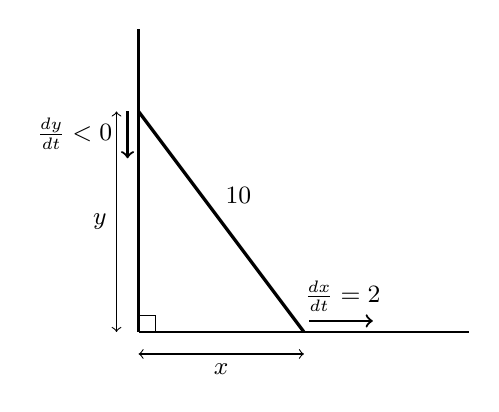
\begin{tikzpicture}[scale=0.35, every node/.style={font=\small}]
  % wall and floor
  \draw[thick] (0,0) -- (0,11);
  \draw[thick] (0,0) -- (12,0);

  % ladder at x=6, y=8
  \draw[very thick] (6,0) -- (0,8);

  % right angle
  \draw (0.6,0) -- (0.6,0.6) -- (0,0.6);

  % labels
  \draw[<->] (0,-0.8) -- (6,-0.8);
  \node[below] at (3,-0.8) {\(x\)};

  \draw[<->] (-0.8,0) -- (-0.8,8);
  \node[left] at (-0.8,4) {\(y\)};

  \node[above right] at (2.8,4.3) {\(10\)};
  \draw[->, thick] (6.2,0.4) -- (8.5,0.4);
  \node[above] at (7.4,0.4) {\(\frac{dx}{dt}=2\)};

  \draw[->, thick] (-0.4,8) -- (-0.4,6.3);
  \node[left] at (-0.6,7.2) {\(\frac{dy}{dt}<0\)};
\end{tikzpicture}
\caption{The ladder length is fixed, so \(x^2+y^2=100\).  The changing lengths \(x\) and \(y\) have related rates.}
\label{fig:related-rates-ladder}
\end{figure}

\paragraph{Example: a growing shadow.}
A \(6\)-foot person walks away from a \(15\)-foot lamp post at

\[
4\text{ ft/s}.
\]

How fast is the tip of the person's shadow moving?

Let

\[
x(t)=\text{distance from the lamp post to the person},
\]

\[
s(t)=\text{length of the shadow},
\]

and

\[
p(t)=x(t)+s(t)=\text{distance from the lamp post to the tip of the shadow}.
\]

We are given

\[
\frac{dx}{dt}=4.
\]

The similar triangles give

\[
\frac{15}{x+s}=\frac{6}{s}.
\]

Cross-multiply:

\[
15s=6(x+s).
\]

So

\[
15s=6x+6s,
\]

hence

\[
9s=6x,
\]

and therefore

\[
s=\frac23x.
\]

Differentiate:

\[
\frac{ds}{dt}=\frac23\frac{dx}{dt}.
\]

Since \(\frac{dx}{dt}=4\),

\[
\frac{ds}{dt}=\frac23(4)=\frac83.
\]

The tip of the shadow is at

\[
p=x+s.
\]

Therefore

\[
\frac{dp}{dt}
=
\frac{dx}{dt}+\frac{ds}{dt}
=
4+\frac83
=
\boxed{\frac{20}{3}}
\]

feet per second.

The tip of the shadow moves faster than the person because the shadow is stretching
while the person moves.

\begin{figure}[h]
\centering
\begin{tikzpicture}[xscale=0.42, yscale=0.42, every node/.style={font=\small}]
  % ground
  \draw[thick] (0,0) -- (22,0);

  % lamp
  \draw[very thick] (0,0) -- (0,15);
  \draw[fill=gray!20] (-0.7,15) rectangle (0.7,16);
  \node[left] at (0,7.5) {\(15\)};

  % person
  \draw[very thick] (9,0) -- (9,6);
  \node[right] at (9,3) {\(6\)};

  % light ray
  \draw[thick] (0,15) -- (15,0);

  % labels
  \draw[<->] (0,-1) -- (9,-1);
  \node[below] at (4.5,-1) {\(x\)};

  \draw[<->] (9,-1) -- (15,-1);
  \node[below] at (12,-1) {\(s\)};

  \draw[<->] (0,-2.1) -- (15,-2.1);
  \node[below] at (7.5,-2.1) {\(p=x+s\)};

  \draw[->, thick] (9.4,0.8) -- (11.5,0.8);
  \node[above] at (10.6,0.8) {\(\frac{dx}{dt}=4\)};
\end{tikzpicture}
\caption{Similar triangles relate the person's position \(x\), the shadow length \(s\), and the tip position \(p=x+s\).}
\label{fig:related-rates-shadow}
\end{figure}

\paragraph{Example: water in a cone.}
An inverted cone has height \(12\) feet and radius \(4\) feet at the top.  Water flows into
the cone at

\[
2\text{ ft}^3/\text{min}.
\]

How fast is the water level rising when the water height is \(6\) feet?

Let

\[
h(t)=\text{height of the water},
\]

\[
r(t)=\text{radius of the water surface},
\]

and

\[
V(t)=\text{volume of water}.
\]

The volume of a cone is

\[
V=\frac13\pi r^2h.
\]

But this formula contains two changing variables, \(r\) and \(h\).  We need one relation
between them.

The water cone is similar to the full tank cone, so

\[
\frac{r}{h}=\frac{4}{12}=\frac13.
\]

Thus

\[
r=\frac{h}{3}.
\]

Substitute into the volume formula:

\[
V
=
\frac13\pi\left(\frac{h}{3}\right)^2h
=
\frac{\pi}{27}h^3.
\]

Differentiate with respect to time:

\[
\frac{dV}{dt}
=
\frac{\pi}{9}h^2\frac{dh}{dt}.
\]

Now use

\[
\frac{dV}{dt}=2,
\qquad
h=6.
\]

Then

\[
2=
\frac{\pi}{9}(6)^2\frac{dh}{dt}
=
4\pi\frac{dh}{dt}.
\]

Therefore

\[
\boxed{
\frac{dh}{dt}=\frac{1}{2\pi}
}
\]

feet per minute.

\begin{figure}[h]
\centering
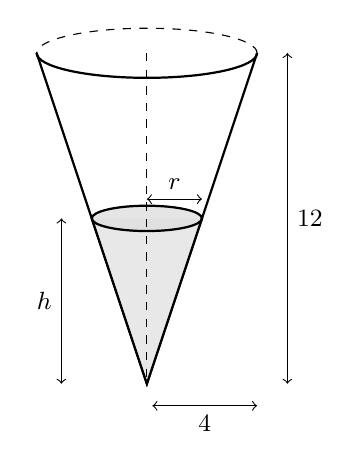
\begin{tikzpicture}[scale=0.7, every node/.style={font=\small}]
  % outer cone
  \draw[thick] (-2,0) -- (0,-6) -- (2,0);
  \draw[thick] (-2,0) arc[start angle=180,end angle=360,x radius=2,y radius=0.45];
  \draw[dashed] (2,0) arc[start angle=0,end angle=180,x radius=2,y radius=0.45];

  % water level at h=3 from vertex
  \draw[fill=gray!18] (-1,-3) -- (0,-6) -- (1,-3);
  \draw[fill=gray!25, opacity=0.8] (0,-3) ellipse (1 and 0.23);
  \draw[thick] (-1,-3) -- (0,-6) -- (1,-3);
  \draw[thick] (0,-3) ellipse (1 and 0.23);

  % axes and measurements
  \draw[dashed] (0,0) -- (0,-6);
  \draw[<->] (2.55,0) -- (2.55,-6);
  \node[right] at (2.55,-3) {\(12\)};

  \draw[<->] (0.1,-6.4) -- (2,-6.4);
  \node[below] at (1.05,-6.4) {\(4\)};

  \draw[<->] (-1.55,-3) -- (-1.55,-6);
  \node[left] at (-1.55,-4.5) {\(h\)};

  \draw[<->] (0,-2.65) -- (1,-2.65);
  \node[above] at (0.5,-2.65) {\(r\)};
\end{tikzpicture}
\caption{Similar triangles give \(r/h=4/12\), so the cone volume can be written using \(h\) alone.}
\label{fig:related-rates-cone}
\end{figure}

\subsection{Units as a guardrail}
\label{subsec:units-guardrail-related-rates}

Related rates problems are easy to damage by a small algebra mistake.  Units help catch
many of those mistakes.

In the balloon problem,

\[
\frac{dV}{dt}
\]

had units

\[
\text{cm}^3/\text{s},
\]

while

\[
4\pi r^2\frac{dr}{dt}
\]

had units

\[
\text{cm}^2\cdot \frac{\text{cm}}{\text{s}}
=
\text{cm}^3/\text{s}.
\]

The units match.

In the ladder problem,

\[
2x\frac{dx}{dt}+2y\frac{dy}{dt}=0.
\]

Both terms have units

\[
\text{ft}\cdot\frac{\text{ft}}{\text{s}}
=
\text{ft}^2/\text{s}.
\]

The units match because we differentiated an equation whose terms had units of square
feet.

Signs are also part of the meaning.

\[
\frac{dx}{dt}>0
\]

means \(x\) is increasing.  In the ladder problem,

\[
\frac{dy}{dt}<0
\]

means \(y\) is decreasing.  If a result says the ladder top is moving ``down'' but gives
a positive \(\frac{dy}{dt}\), something has been mislabeled or misread.

\begin{quote}
\textbf{A rate is not just a number.}

A rate carries units and direction.  Before trusting an answer, ask:

\[
\text{Does the sign make sense?}
\]

\[
\text{Do the units make sense?}
\]

\[
\text{Was the equation differentiated before instant-specific values were substituted?}
\]
\end{quote}

Related rates tell how quantities change together.  The next problem is different.  Instead
of asking how fast something changes, we ask which choice is best.

\section{Optimization problems}
\label{sec:optimization-problems}

The previous chapter taught us how to find high and low points of a function.  Optimization
turns that skill into a method for solving word problems.

A real question rarely arrives as

\[
\text{maximize } f(x).
\]

It arrives as a sentence:

\[
\text{Build the largest box from this sheet of cardboard.}
\]

\[
\text{Use the least metal for this can.}
\]

\[
\text{Enclose the most area with this much fence.}
\]

The first task is not calculus.  The first task is translation.

\[
\text{situation}
\quad\longrightarrow\quad
\text{function}
\quad\longrightarrow\quad
\text{derivative}
\quad\longrightarrow\quad
\text{decision}.
\]

\subsection{Translating a word problem into a function}
\label{subsec:translating-word-problem-function}

A farmer has \(200\) meters of fencing and wants to enclose a rectangular field along a
straight river.  The river forms one side of the rectangle, so fencing is needed only for
the other three sides.

What dimensions give the largest area?

Let

\[
x=\text{the width perpendicular to the river}
\]

and

\[
y=\text{the length parallel to the river}.
\]

The fencing is used for two widths and one length:

\[
2x+y=200.
\]

The area is

\[
A=xy.
\]

We want to maximize \(A\), but right now \(A\) uses two variables.  Use the constraint

\[
2x+y=200
\]

to solve for \(y\):

\[
y=200-2x.
\]

Then

\[
A(x)=x(200-2x)=200x-2x^2.
\]

Now the problem is a one-variable calculus problem.

The physical domain is

\[
0\le x\le 100.
\]

If \(x=0\), the rectangle has no width.  If \(x=100\), then \(y=0\).  Both give area \(0\).
For \(0<x<100\), the rectangle has positive area.

Differentiate:

\[
A'(x)=200-4x.
\]

Set the derivative equal to \(0\):

\[
200-4x=0.
\]

Thus

\[
x=50.
\]

Then

\[
y=200-2(50)=100.
\]

The maximum area occurs when

\[
\boxed{
x=50,\qquad y=100.
}
\]

The farmer should build a field \(50\) meters wide and \(100\) meters long.

\begin{figure}[h]
\centering
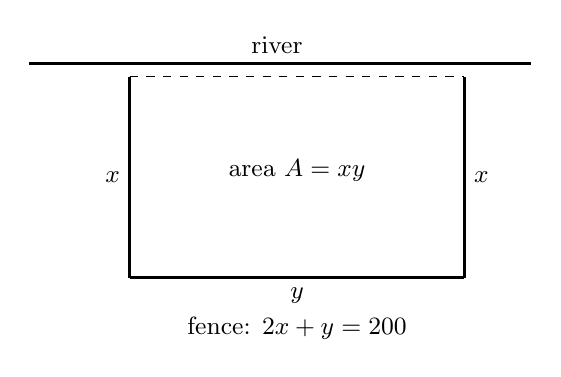
\begin{tikzpicture}[scale=0.85, every node/.style={font=\small}]
  % river
  \draw[very thick] (-0.5,3.2) -- (7,3.2);
  \node[above] at (3.2,3.2) {river};

  % field fence
  \draw[very thick] (1,0) -- (1,3);
  \draw[very thick] (1,0) -- (6,0);
  \draw[very thick] (6,0) -- (6,3);
  \draw[dashed] (1,3) -- (6,3);

  \node[left] at (1,1.5) {\(x\)};
  \node[right] at (6,1.5) {\(x\)};
  \node[below] at (3.5,0) {\(y\)};

  \node at (3.5,1.6) {area \(A=xy\)};
  \node[below] at (3.5,-0.45) {fence: \(2x+y=200\)};
\end{tikzpicture}
\caption{The river supplies one side, so the fencing constraint is \(2x+y=200\).}
\label{fig:fence-river-optimization}
\end{figure}

\begin{quote}
\textbf{The optimization translation.}

\[
\begin{array}{ll}
\text{objective} & \text{the quantity to maximize or minimize} \\
\text{constraint} & \text{the condition that limits the choices} \\
\text{domain} & \text{the physically meaningful values of the variable}
\end{array}
\]
\end{quote}

In the fencing problem, the objective was area, the constraint was the amount of fencing,
and the domain came from requiring nonnegative side lengths.

\subsection{Constraints in one variable}
\label{subsec:constraints-one-variable}

Many optimization problems begin with several quantities.  The constraint is what lets us
reduce to one variable.

The general pattern is:

\[
\text{objective } Q=Q(x,y)
\]

together with

\[
\text{constraint relating }x\text{ and }y.
\]

Use the constraint to write

\[
y=\text{a formula in }x.
\]

Then

\[
Q=Q(x)
\]

becomes a one-variable function.

\begin{quote}
\textbf{Optimization workflow.}

\[
\begin{array}{ll}
\text{1.} & \text{Identify the quantity to optimize.}\\
\text{2.} & \text{Name the variables.}\\
\text{3.} & \text{Write the objective function.}\\
\text{4.} & \text{Write the constraint.}\\
\text{5.} & \text{Use the constraint to get one variable.}\\
\text{6.} & \text{Find the physical domain.}\\
\text{7.} & \text{Use derivatives and endpoint checks.}\\
\text{8.} & \text{Translate the answer back into the problem.}
\end{array}
\]
\end{quote}

The domain is not optional.  It is part of the model.

A critical number outside the physical domain is not a possible solution.  An endpoint
inside the domain may be the best solution.

\subsection{Geometry: boxes, fences, cans, and light paths}
\label{subsec:geometry-optimization}

Geometry problems are good training because the constraints are visible.

\paragraph{Example: the largest open box from a square sheet.}
A square sheet of cardboard is \(12\) inches by \(12\) inches.  Equal squares of side
length \(x\) are cut from the four corners.  The sides are folded up to make an open box.

What value of \(x\) gives the largest volume?

After cutting, the base has side length

\[
12-2x.
\]

The height is

\[
x.
\]

So the volume is

\[
V(x)=x(12-2x)^2.
\]

The physical domain is

\[
0\le x\le 6.
\]

At \(x=0\), no box is formed.  At \(x=6\), the base has side length \(0\).  Both endpoints
give volume \(0\).

Differentiate:

\[
V(x)=x(12-2x)^2.
\]

Using the product and chain rules,

\[
V'(x)
=
(12-2x)^2+x\cdot 2(12-2x)(-2).
\]

Factor:

\[
V'(x)
=
(12-2x)\bigl((12-2x)-4x\bigr).
\]

Thus

\[
V'(x)
=
(12-2x)(12-6x).
\]

The critical numbers are

\[
x=6
\qquad\text{and}\qquad
x=2.
\]

The number \(x=6\) is an endpoint.  The interior critical number is \(x=2\).

Check the volumes:

\[
V(0)=0,
\]

\[
V(2)=2(12-4)^2=2(8)^2=128,
\]

\[
V(6)=0.
\]

Therefore the largest volume occurs at

\[
\boxed{x=2}
\]

inches.  The box dimensions are

\[
8\text{ in}\times 8\text{ in}\times 2\text{ in}.
\]

\begin{figure}[h]
\centering
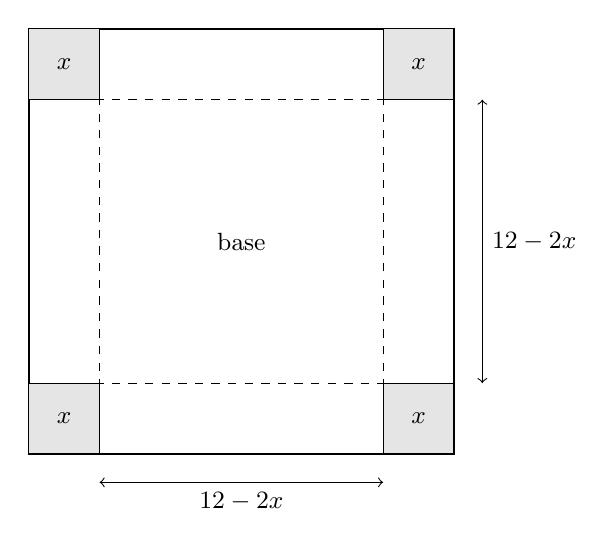
\begin{tikzpicture}[scale=0.45, every node/.style={font=\small}]
  % square sheet
  \draw[thick] (0,0) rectangle (12,12);

  % corner cuts
  \draw[fill=gray!20] (0,0) rectangle (2,2);
  \draw[fill=gray!20] (10,0) rectangle (12,2);
  \draw[fill=gray!20] (0,10) rectangle (2,12);
  \draw[fill=gray!20] (10,10) rectangle (12,12);

  % fold lines
  \draw[dashed] (2,0) -- (2,12);
  \draw[dashed] (10,0) -- (10,12);
  \draw[dashed] (0,2) -- (12,2);
  \draw[dashed] (0,10) -- (12,10);

  % labels
  \node at (1,1) {\(x\)};
  \node at (11,1) {\(x\)};
  \node at (1,11) {\(x\)};
  \node at (11,11) {\(x\)};

  \draw[<->] (2,-0.8) -- (10,-0.8);
  \node[below] at (6,-0.8) {\(12-2x\)};

  \draw[<->] (12.8,2) -- (12.8,10);
  \node[right] at (12.8,6) {\(12-2x\)};

  \node at (6,6) {base};
\end{tikzpicture}
\caption{Cutting out four squares of side length \(x\) leaves an open box with volume \(V=x(12-2x)^2\).}
\label{fig:open-box-cardboard}
\end{figure}

\paragraph{Example: the least material for a closed can.}
A closed cylindrical can must hold volume \(V_0\).  What shape uses the least surface
area?

Let

\[
r=\text{radius}
\]

and

\[
h=\text{height}.
\]

The volume constraint is

\[
\pi r^2h=V_0.
\]

The surface area of a closed cylinder is

\[
S=2\pi r^2+2\pi rh.
\]

Use the constraint to solve for \(h\):

\[
h=\frac{V_0}{\pi r^2}.
\]

Substitute into \(S\):

\[
S(r)
=
2\pi r^2+2\pi r\left(\frac{V_0}{\pi r^2}\right).
\]

So

\[
S(r)=2\pi r^2+\frac{2V_0}{r},
\qquad r>0.
\]

Differentiate:

\[
S'(r)=4\pi r-\frac{2V_0}{r^2}.
\]

Set \(S'(r)=0\):

\[
4\pi r-\frac{2V_0}{r^2}=0.
\]

Multiply by \(r^2\):

\[
4\pi r^3-2V_0=0.
\]

Thus

\[
2\pi r^3=V_0.
\]

Now compute the corresponding height:

\[
h=\frac{V_0}{\pi r^2}.
\]

Since \(V_0=2\pi r^3\),

\[
h=\frac{2\pi r^3}{\pi r^2}=2r.
\]

Therefore the least-material closed can satisfies

\[
\boxed{
h=2r.
}
\]

The height equals the diameter.

\begin{figure}[h]
\centering
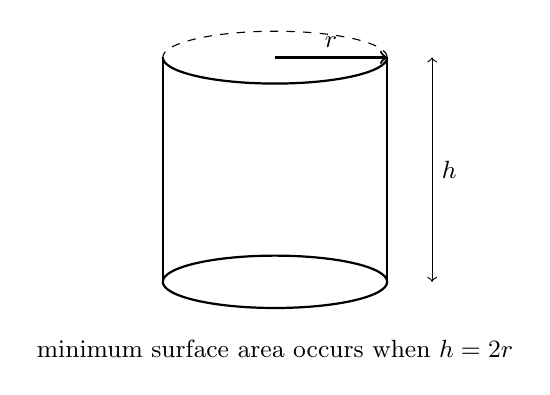
\begin{tikzpicture}[scale=0.95, every node/.style={font=\small}]
  % cylinder
  \draw[thick] (-1.5,1.5) arc[start angle=180,end angle=360,x radius=1.5,y radius=0.35];
  \draw[dashed] (1.5,1.5) arc[start angle=0,end angle=180,x radius=1.5,y radius=0.35];
  \draw[thick] (-1.5,-1.5) arc[start angle=180,end angle=360,x radius=1.5,y radius=0.35];
  \draw[thick] (-1.5,-1.5) arc[start angle=180,end angle=0,x radius=1.5,y radius=0.35];
  \draw[thick] (-1.5,1.5) -- (-1.5,-1.5);
  \draw[thick] (1.5,1.5) -- (1.5,-1.5);

  % radius
  \draw[->, thick] (0,1.5) -- (1.5,1.5);
  \node[above] at (0.75,1.5) {\(r\)};

  % height
  \draw[<->] (2.1,1.5) -- (2.1,-1.5);
  \node[right] at (2.1,0) {\(h\)};

  \node at (0,-2.4) {minimum surface area occurs when \(h=2r\)};
\end{tikzpicture}
\caption{For a closed cylinder with fixed volume, the surface area is minimized when height equals diameter.}
\label{fig:closed-can-min-area}
\end{figure}

A second derivative check confirms this critical point is a minimum:

\[
S''(r)=4\pi+\frac{4V_0}{r^3}>0.
\]

So \(S\) is concave up at every positive \(r\).  The critical point is the least surface area.

\paragraph{Example: the shortest reflected path.}
A point \(A\) is located \(a\) units above a straight mirror, and a point \(B\) is located
\(b\) units above the same mirror.  Their horizontal separation is \(L\).  A light ray travels
from \(A\) to the mirror and then to \(B\).  Where should it hit the mirror to make the
total distance as small as possible?

Place the mirror on the \(x\)-axis.  Let

\[
A=(0,a),
\qquad
B=(L,b),
\]

and let the reflection point be

\[
P=(x,0).
\]

The total distance is

\[
D(x)=\sqrt{x^2+a^2}+\sqrt{(L-x)^2+b^2}.
\]

The physical domain is

\[
0\le x\le L.
\]

Differentiate:

\[
D'(x)
=
\frac{x}{\sqrt{x^2+a^2}}
-
\frac{L-x}{\sqrt{(L-x)^2+b^2}}.
\]

At the shortest path, an interior critical point must satisfy

\[
\frac{x}{\sqrt{x^2+a^2}}
=
\frac{L-x}{\sqrt{(L-x)^2+b^2}}.
\]

Both sides are positive, so square:

\[
\frac{x^2}{x^2+a^2}
=
\frac{(L-x)^2}{(L-x)^2+b^2}.
\]

Cross-multiply:

\[
x^2\bigl((L-x)^2+b^2\bigr)
=
(L-x)^2(x^2+a^2).
\]

Cancel the matching term \(x^2(L-x)^2\):

\[
b^2x^2=a^2(L-x)^2.
\]

Taking positive square roots gives

\[
bx=a(L-x).
\]

Therefore

\[
(a+b)x=aL,
\]

so

\[
\boxed{
x=\frac{aL}{a+b}.
}
\]

This condition is the familiar reflection rule: the incoming and outgoing angles are equal.
The derivative has found the law of reflection from a shortest-path principle.

\begin{figure}[h]
\centering
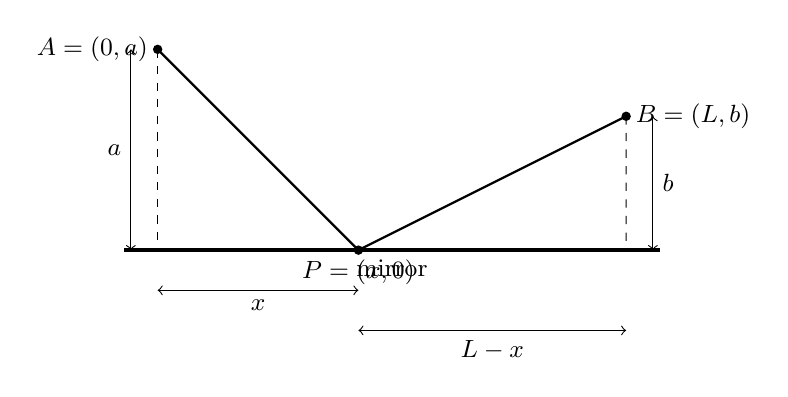
\begin{tikzpicture}[scale=0.85, every node/.style={font=\small}]
  % mirror
  \draw[very thick] (-0.5,0) -- (7.5,0);
  \node[below] at (3.5,0) {mirror};

  % points
  \coordinate (A) at (0,3);
  \coordinate (P) at (3,0);
  \coordinate (B) at (7,2);

  \fill (A) circle (2pt);
  \fill (P) circle (2pt);
  \fill (B) circle (2pt);

  \node[left] at (A) {\(A=(0,a)\)};
  \node[below] at (P) {\(P=(x,0)\)};
  \node[right] at (B) {\(B=(L,b)\)};

  % paths
  \draw[thick] (A) -- (P) -- (B);

  % heights
  \draw[dashed] (A) -- (0,0);
  \draw[dashed] (B) -- (7,0);

  \draw[<->] (0,-0.6) -- (3,-0.6);
  \node[below] at (1.5,-0.6) {\(x\)};

  \draw[<->] (3,-1.2) -- (7,-1.2);
  \node[below] at (5,-1.2) {\(L-x\)};

  \draw[<->] (-0.4,0) -- (-0.4,3);
  \node[left] at (-0.4,1.5) {\(a\)};

  \draw[<->] (7.4,0) -- (7.4,2);
  \node[right] at (7.4,1) {\(b\)};
\end{tikzpicture}
\caption{The total path length is \(D(x)=\sqrt{x^2+a^2}+\sqrt{(L-x)^2+b^2}\).}
\label{fig:reflection-shortest-path}
\end{figure}

\subsection{Endpoint checks and physical feasibility}
\label{subsec:endpoint-checks-physical-feasibility}

Optimization problems are not finished when we find a critical number.

A critical number is a candidate.  It may give a maximum, a minimum, neither, or it may
not be physically allowed.

The correct conclusion depends on the domain.

\begin{quote}
\textbf{Closed interval method for applications.}

If the objective function is continuous on a closed interval, then:

\[
\begin{array}{ll}
\text{1.} & \text{Find the critical numbers inside the interval.}\\
\text{2.} & \text{Evaluate the objective function at those critical numbers.}\\
\text{3.} & \text{Evaluate the objective function at the endpoints.}\\
\text{4.} & \text{Compare the values.}
\end{array}
\]
\end{quote}

In the open-box problem, the domain was

\[
0\le x\le 6.
\]

The endpoints gave

\[
V(0)=0,
\qquad
V(6)=0.
\]

The interior critical point gave

\[
V(2)=128.
\]

So \(x=2\) gave the absolute maximum.

But endpoints do not always lose.  If a problem asks for a minimum, an endpoint may win.
If a domain is open, the best value may not be attained at all.  If a critical point lies outside
the physical domain, it is irrelevant.

\paragraph{Warning example: a critical point outside the domain.}
Suppose a company models profit from selling \(q\) units by

\[
P(q)=-q^2+40q-300.
\]

The derivative is

\[
P'(q)=-2q+40.
\]

The critical point is

\[
q=20.
\]

If the company can produce any number of units between \(0\) and \(50\), then \(q=20\)
is a real candidate.  But if a contract requires

\[
30\le q\le 50,
\]

then \(q=20\) is not physically allowed.  On the interval \([30,50]\),

\[
P'(q)=-2q+40<0.
\]

So \(P\) is decreasing throughout the allowed interval.  The maximum allowed profit occurs
at the endpoint

\[
q=30.
\]

The derivative found the best point for the wrong domain.

\begin{quote}
\textbf{The domain is part of the problem.}

A formula alone does not know what choices are possible.  The domain tells the formula
which choices are allowed.
\end{quote}

Related rates asked how fast quantities change together.  Optimization asked which choice
is best.  Both depended on building a model and then reading a derivative.

But real measurements are rarely exact.  A radius may be \(3\) cm only to the nearest
millimeter.  A length may have a small error.  The next question is not the best exact
choice, but how sensitive an answer is to small changes.
\section{Linear approximation in applications}
\label{sec:linear-approximation-applications}

Optimization asked for the best choice.  Related rates asked how fast quantities
change together.

Measurements ask a quieter question.

\[
\text{If the input is a little wrong, how wrong is the output?}
\]

A radius may be measured only to the nearest millimeter.  An angle may be off by
one degree.  A price model may be only an approximation.  Calculus gives a first
answer through the tangent line.

Recall the local linear approximation:

\[
f(a+\Delta x)\approx f(a)+f'(a)\Delta x.
\]

The derivative is the multiplier that turns a small input change into a small output
change.

\[
\Delta y\approx f'(a)\Delta x.
\]

That is the practical meaning of the derivative in this section.

\subsection{Estimating hard numbers quickly}
\label{subsec:estimating-hard-numbers-quickly}

Some numbers are hard to compute exactly, but close to numbers we know well.

For example, \(\sqrt{26}\) is close to \(\sqrt{25}\).  Since

\[
\sqrt{25}=5,
\]

we can use the tangent line to

\[
f(x)=\sqrt{x}
\]

at

\[
x=25.
\]

The derivative is

\[
f'(x)=\frac{1}{2\sqrt{x}}.
\]

So

\[
f'(25)=\frac{1}{2\cdot5}=\frac{1}{10}.
\]

The linear approximation at \(x=25\) is

\[
L(x)=f(25)+f'(25)(x-25).
\]

Thus

\[
L(x)=5+\frac{1}{10}(x-25).
\]

For \(x=26\),

\[
\sqrt{26}=f(26)\approx L(26)
=
5+\frac{1}{10}
=
5.1.
\]

So

\[
\boxed{\sqrt{26}\approx 5.1.}
\]

This is close.  In fact,

\[
5.1^2=26.01,
\]

so \(5.1\) is slightly larger than \(\sqrt{26}\).

\begin{figure}[h]
\centering
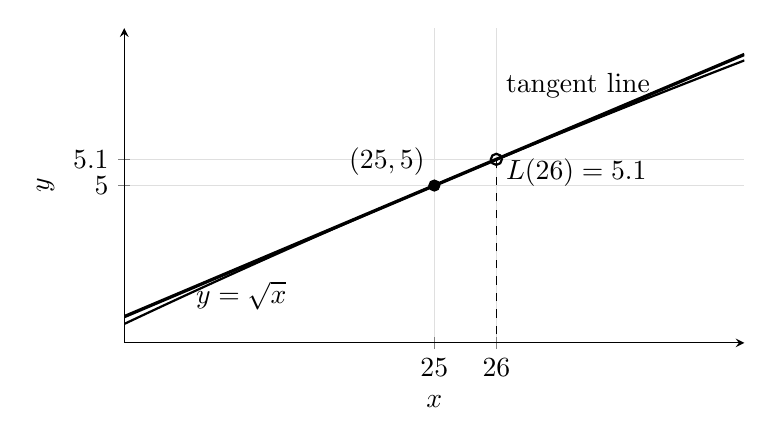
\begin{tikzpicture}
\begin{axis}[
    width=0.78\textwidth,
    height=0.46\textwidth,
    xmin=20, xmax=30,
    ymin=4.4, ymax=5.6,
    axis lines=left,
    xlabel={\(x\)},
    ylabel={\(y\)},
    xtick={25,26},
    ytick={5,5.1},
    grid=both,
    grid style={line width=.1pt, draw=gray!25},
]
\addplot[thick, domain=20:30, samples=150] {sqrt(x)};
\addplot[very thick, domain=20:30, samples=2] {5+(x-25)/10};
\addplot[only marks, mark=*] coordinates {(25,5)};
\addplot[only marks, mark=o, thick] coordinates {(26,5.1)};
\draw[dashed] (axis cs:26,0) -- (axis cs:26,5.1);
\node[anchor=south east] at (axis cs:25,5) {\((25,5)\)};
\node[anchor=west] at (axis cs:26,5.05) {\(L(26)=5.1\)};
\node[anchor=west] at (axis cs:26,5.38) {tangent line};
\node[anchor=west] at (axis cs:21,4.58) {\(y=\sqrt{x}\)};
\end{axis}
\end{tikzpicture}
\caption{Near \(x=25\), the tangent line to \(y=\sqrt{x}\) gives a quick estimate of \(\sqrt{x}\).}
\label{fig:linear-approx-sqrt26}
\end{figure}

The general name for this tangent-line function is the \emph{linearization}.

\begin{quote}
\textbf{Linearization.}
If \(f\) is differentiable at \(a\), then the linearization of \(f\) at \(a\) is

\[
\boxed{
L(x)=f(a)+f'(a)(x-a).
}
\]

For \(x\) close to \(a\),

\[
f(x)\approx L(x).
\]
\end{quote}

The word ``close'' matters.  A tangent line is a local model.  It is meant for nearby
inputs.

\paragraph{Example.}
Use linear approximation to estimate

\[
\sqrt[3]{65}.
\]

Let

\[
f(x)=\sqrt[3]{x}=x^{1/3}.
\]

The number \(65\) is close to \(64\), and

\[
\sqrt[3]{64}=4.
\]

So take

\[
a=64.
\]

The derivative is

\[
f'(x)=\frac13x^{-2/3}.
\]

At \(x=64\),

\[
f'(64)=\frac13\cdot\frac{1}{64^{2/3}}.
\]

Since

\[
64^{1/3}=4,
\]

we have

\[
64^{2/3}=4^2=16.
\]

Therefore

\[
f'(64)=\frac{1}{48}.
\]

The linearization is

\[
L(x)=4+\frac{1}{48}(x-64).
\]

For \(x=65\),

\[
\sqrt[3]{65}\approx 4+\frac{1}{48}
=
\frac{193}{48}
\approx 4.0208.
\]

\paragraph{A warning about going too far.}
Linear approximation is local.  For

\[
f(x)=\frac{1}{1-x},
\]

the linearization at \(x=0\) is

\[
L(x)=1+x.
\]

At \(x=0.05\),

\[
f(0.05)=\frac{1}{0.95}\approx 1.0526,
\]

while

\[
L(0.05)=1.05.
\]

That is useful.

At \(x=0.9\),

\[
f(0.9)=10,
\]

but

\[
L(0.9)=1.9.
\]

That is not useful.  The tangent line knew the function near \(0\), not near the
vertical asymptote at \(x=1\).

\begin{quote}
\textbf{Local means local.}

A tangent line is a good model only while the graph has not had time to bend much.
\end{quote}

\subsection{Error propagation}
\label{subsec:error-propagation}

Suppose an input \(x\) is measured with a small error.  Write the measured change as

\[
\Delta x.
\]

If

\[
y=f(x),
\]

then the exact output change is

\[
\Delta y=f(x+\Delta x)-f(x).
\]

The derivative gives the approximation

\[
\Delta y\approx f'(x)\Delta x.
\]

This is often written using differentials:

\[
dy=f'(x)\,dx.
\]

When we use the differential to estimate an actual small change, we set

\[
dx=\Delta x
\]

and then use

\[
\boxed{
\Delta y\approx dy.
}
\]

\paragraph{Example: error in the volume of a sphere.}
A spherical ball has radius measured as

\[
r=3.00\text{ cm},
\]

with possible measurement error

\[
|dr|\le 0.02\text{ cm}.
\]

Estimate the possible error in the computed volume.

The volume of a sphere is

\[
V=\frac43\pi r^3.
\]

Differentiate:

\[
dV=4\pi r^2\,dr.
\]

At

\[
r=3,
\]

we get

\[
dV=4\pi(3)^2\,dr=36\pi\,dr.
\]

Since

\[
|dr|\le0.02,
\]

the maximum estimated volume error is

\[
|dV|
\le
36\pi(0.02)
=
0.72\pi.
\]

So

\[
\boxed{
|dV|\lesssim 0.72\pi\approx 2.26\text{ cm}^3.
}
\]

The symbol \(\lesssim\) means ``approximately less than or equal to.''  This is an
estimated error bound, not an exact one.

\begin{figure}[h]
\centering
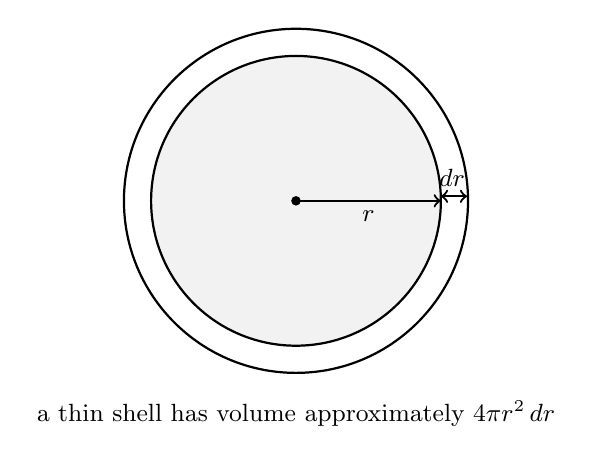
\begin{tikzpicture}[scale=1.15, every node/.style={font=\small}]
  % Cross-section circles
  \draw[fill=gray!10, thick] (0,0) circle (1.6);
  \draw[thick] (0,0) circle (1.9);

  % Radius and dr
  \draw[->, thick] (0,0) -- (1.6,0);
  \node[below] at (0.8,0) {\(r\)};

  \draw[<->, thick] (1.6,0.05) -- (1.89,0.05);
  \node[above] at (1.725,0.05) {\(dr\)};

  % Center
  \fill (0,0) circle (1.5pt);

  \node at (0,-2.35) {a thin shell has volume approximately \(4\pi r^2\,dr\)};
\end{tikzpicture}
\caption{For a sphere, \(dV=4\pi r^2\,dr\): surface area times a small change in radius.}
\label{fig:sphere-shell-differential}
\end{figure}

This formula also has a geometric meaning.  Increasing the radius by a small amount
\(dr\) adds a thin shell.  Its volume is approximately

\[
\text{surface area}\times\text{thickness}
=
4\pi r^2\,dr.
\]

That is exactly the differential \(dV\).

\paragraph{Absolute error form.}
If \(x\) has maximum possible error

\[
|\Delta x|\le E_x,
\]

then the output error is estimated by

\[
\boxed{
|\Delta y|\approx |f'(x)|\,|\Delta x|.
}
\]

So a practical estimate is

\[
\boxed{
|\Delta y|\lesssim |f'(x)|E_x.
}
\]

The derivative acts as an error multiplier.

\subsection{Relative and percentage error}
\label{subsec:relative-percentage-error}

Absolute error tells the size of the error in the units of the quantity.  Relative error
compares the error to the size of the quantity itself.

If \(y\neq0\), then

\[
\text{relative error}
=
\frac{|\Delta y|}{|y|}.
\]

The percentage error is

\[
\text{percentage error}
=
\frac{|\Delta y|}{|y|}\cdot100\%.
\]

For estimates, we use differentials:

\[
\frac{|\Delta y|}{|y|}
\approx
\frac{|dy|}{|y|}.
\]

\paragraph{Example: error in the area of a disk.}
A circular disk has measured radius

\[
r=24\text{ cm},
\]

with possible measurement error

\[
|dr|\le0.2\text{ cm}.
\]

The area is

\[
A=\pi r^2.
\]

So

\[
dA=2\pi r\,dr.
\]

At \(r=24\),

\[
|dA|
\le
2\pi(24)(0.2)
=
9.6\pi.
\]

Thus the maximum estimated area error is

\[
\boxed{
|dA|\lesssim 9.6\pi\approx30.2\text{ cm}^2.
}
\]

Now compute relative error:

\[
\frac{|dA|}{A}
=
\frac{|2\pi r\,dr|}{\pi r^2}
=
2\frac{|dr|}{r}.
\]

Substitute the values:

\[
\frac{|dA|}{A}
\lesssim
2\frac{0.2}{24}
=
\frac{0.4}{24}
=
\frac{1}{60}.
\]

As a percentage,

\[
\frac{1}{60}\cdot100\%
\approx
1.67\%.
\]

So the radius error of about

\[
\frac{0.2}{24}\cdot100\%\approx0.83\%
\]

produces an area error of about

\[
1.67\%.
\]

The percentage error doubled because area depends on the square of radius.

\paragraph{Power laws.}
Suppose

\[
y=Cx^n,
\]

where \(C\) and \(n\) are constants.  Then

\[
dy=nCx^{n-1}\,dx.
\]

Divide by

\[
y=Cx^n:
\]

\[
\frac{dy}{y}
=
\frac{nCx^{n-1}\,dx}{Cx^n}
=
n\frac{dx}{x}.
\]

So

\[
\boxed{
\frac{dy}{y}\approx n\frac{dx}{x}.
}
\]

For a power law, the relative output error is approximately \(n\) times the relative
input error.

\[
\begin{array}{c|c}
\textbf{quantity} & \textbf{relative error rule} \\ \hline
A=\pi r^2 & \dfrac{dA}{A}=2\dfrac{dr}{r} \\[8pt]
V=\dfrac43\pi r^3 & \dfrac{dV}{V}=3\dfrac{dr}{r} \\[8pt]
y=Cx^n & \dfrac{dy}{y}=n\dfrac{dx}{x}
\end{array}
\]

This is why small measurement errors can grow when a formula contains powers.

\subsection{Sensitivity in measurement}
\label{subsec:sensitivity-in-measurement}

The derivative measures sensitivity.

If

\[
y=f(x),
\]

then

\[
f'(x)
\]

has units

\[
\frac{\text{output units}}{\text{input units}}.
\]

A large value of \(|f'(x)|\) means that a small input error can create a large output
error.  A small value of \(|f'(x)|\) means the output is less sensitive to input error.

\paragraph{Example: measuring height using an angle.}
A surveyor stands

\[
100\text{ m}
\]

from the base of a tower.  The angle of elevation to the top is \(\theta\).  The height
\(H\) of the tower is modeled by

\[
H=100\tan\theta.
\]

Differentiate:

\[
dH=100\sec^2\theta\,d\theta.
\]

The derivative formula for \(\tan\theta\) assumes that \(\theta\) is measured in radians.
A one-degree error is

\[
1^\circ=\frac{\pi}{180}
\]

radians.

If

\[
\theta=45^\circ,
\]

then

\[
\sec^2(45^\circ)=2.
\]

So a one-degree measurement error gives

\[
|dH|
\approx
100(2)\frac{\pi}{180}
\approx
3.49\text{ m}.
\]

If

\[
\theta=80^\circ,
\]

then

\[
\sec^2(80^\circ)\approx33.2.
\]

The same one-degree error gives

\[
|dH|
\approx
100(33.2)\frac{\pi}{180}
\approx
57.9\text{ m}.
\]

The distance error is the same.  The angle error is the same.  The sensitivity is not
the same.  Near a vertical angle, the tangent function changes very quickly.

\begin{figure}[h]
\centering
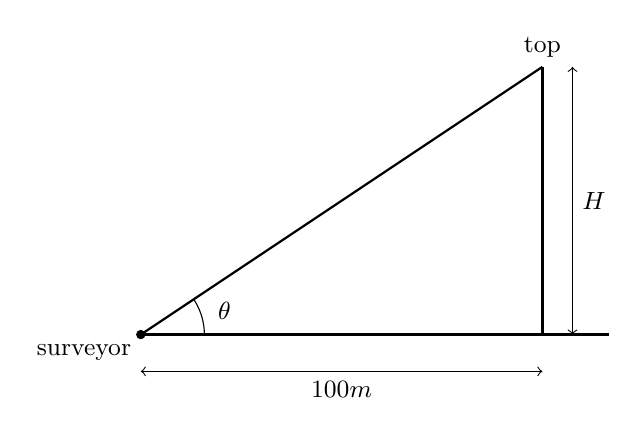
\begin{tikzpicture}[scale=0.85, every node/.style={font=\small}]
  % Ground and tower
  \draw[thick] (0,0) -- (7,0);
  \draw[very thick] (6,0) -- (6,4);

  % Line of sight
  \draw[thick] (0,0) -- (6,4);

  % Labels
  \draw[<->] (0,-0.55) -- (6,-0.55);
  \node[below] at (3,-0.55) {\(100\text{ m}\)};

  \draw[<->] (6.45,0) -- (6.45,4);
  \node[right] at (6.45,2) {\(H\)};

  \draw (0.95,0) arc[start angle=0,end angle=33.69,radius=0.95];
  \node at (1.25,0.35) {\(\theta\)};

  \fill (0,0) circle (2pt);
  \node[below left] at (0,0) {surveyor};

  \node[above] at (6,4) {top};
\end{tikzpicture}
\caption{The model \(H=100\tan\theta\) becomes very sensitive when \(\theta\) is large.}
\label{fig:angle-height-sensitivity}
\end{figure}

\begin{quote}
\textbf{Sensitivity.}

For \(y=f(x)\), the size of \(|f'(x)|\) tells how strongly errors in \(x\) are amplified
into errors in \(y\).
\end{quote}

Linear approximation gives us three related calculations:

\[
\begin{array}{ccl}
\text{estimate output change} &:& \Delta y\approx f'(x)\Delta x,\\[4pt]
\text{estimate input change} &:& \Delta x\approx \dfrac{\Delta y}{f'(x)},\\[10pt]
\text{estimate sensitivity} &:& \left|\dfrac{\Delta y}{\Delta x}\right|\approx |f'(x)|.
\end{array}
\]

So far we have mostly used the first and third.  The second one is about to become a
method for solving equations.

If \(f(x)\) is not zero, how far should we move \(x\) so that \(f(x)\) becomes zero?
The tangent line gives the first guess.  Repeating that guess gives Newton's method.

\section{Newton's method}
\label{sec:newtons-method}

Linear approximation estimates a function by a line.

Newton's method uses that line to solve an equation.

Suppose we want to solve

\[
f(x)=0.
\]

The solution is a point where the graph of \(f\) crosses the \(x\)-axis.  If we already
have a nearby guess \(x_0\), the tangent line at \(x_0\) is often easier to use than the
curve itself.  The tangent line crosses the \(x\)-axis at a new guess.

Then we do it again.

\subsection{Tangent lines as root finders}
\label{subsec:tangent-lines-root-finders}

We begin with a familiar problem:

\[
\sqrt2.
\]

Instead of asking directly for \(\sqrt2\), solve

\[
x^2=2.
\]

Equivalently, find a zero of

\[
f(x)=x^2-2.
\]

A reasonable first guess is

\[
x_0=1.5.
\]

At this point,

\[
f(1.5)=1.5^2-2=2.25-2=0.25,
\]

and

\[
f'(x)=2x,
\]

so

\[
f'(1.5)=3.
\]

The tangent line at \(x_0=1.5\) is

\[
y=f(x_0)+f'(x_0)(x-x_0).
\]

Thus

\[
y=0.25+3(x-1.5).
\]

Newton's idea is to follow this tangent line down to the \(x\)-axis.  Set \(y=0\):

\[
0=0.25+3(x-1.5).
\]

Then

\[
3(x-1.5)=-0.25,
\]

so

\[
x-1.5=-\frac{0.25}{3}=-\frac{1}{12}.
\]

Therefore

\[
x=1.5-\frac{1}{12}
=
\frac32-\frac{1}{12}
=
\frac{17}{12}
\approx1.4166667.
\]

This is already closer to \(\sqrt2\) than \(1.5\).

\begin{figure}[h]
\centering
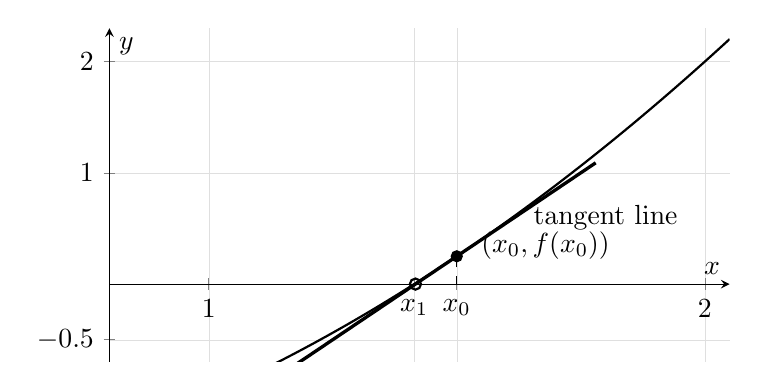
\begin{tikzpicture}
\begin{axis}[
    width=0.78\textwidth,
    height=0.48\textwidth,
    xmin=0.8, xmax=2.05,
    ymin=-0.7, ymax=2.3,
    axis lines=middle,
    xlabel={\(x\)},
    ylabel={\(y\)},
    xtick={1,1.4142,1.5,2},
    xticklabels={\(1\),\(x_1\),\(x_0\),\(2\)},
    ytick={-0.5,0,1,2},
    grid=both,
    grid style={line width=.1pt, draw=gray!25},
]
\addplot[thick, domain=0.8:2.05, samples=150] {x^2-2};
\addplot[very thick, domain=0.95:1.78, samples=2] {0.25+3*(x-1.5)};
\addplot[only marks, mark=*] coordinates {(1.5,0.25)};
\addplot[only marks, mark=o, thick] coordinates {(1.4166667,0)};
\draw[dashed] (axis cs:1.5,0) -- (axis cs:1.5,0.25);
\node[anchor=west] at (axis cs:1.53,0.35) {\((x_0,f(x_0))\)};

\node[anchor=north] at (axis cs:1.8,0.8) {tangent line};
\end{axis}
\end{tikzpicture}
\caption{Newton's method replaces the curve by its tangent line and uses the tangent's \(x\)-intercept as the next guess.}
\label{fig:newton-sqrt2-first-step}
\end{figure}

Now repeat the same process using

\[
x_1=\frac{17}{12}.
\]

Newton's next approximation is

\[
x_2
=
\frac{577}{408}
\approx
1.414215686.
\]

Already the first five decimal places are correct.

\subsection{The iteration formula}
\label{subsec:newton-iteration-formula}

The same tangent-line calculation works for any differentiable function.

Suppose \(x_n\) is the current guess for a zero of \(f\).  The tangent line at \(x_n\) is

\[
y=f(x_n)+f'(x_n)(x-x_n).
\]

Set \(y=0\) to find where this tangent line crosses the \(x\)-axis:

\[
0=f(x_n)+f'(x_n)(x-x_n).
\]

Solve for \(x\):

\[
f'(x_n)(x-x_n)=-f(x_n),
\]

so

\[
x-x_n=-\frac{f(x_n)}{f'(x_n)}.
\]

Therefore

\[
x=x_n-\frac{f(x_n)}{f'(x_n)}.
\]

This is the next guess.

\begin{quote}
\textbf{Newton's method.}
To solve

\[
f(x)=0,
\]

start with an initial guess \(x_0\).  Then define

\[
\boxed{
x_{n+1}
=
x_n-\frac{f(x_n)}{f'(x_n)}
}
\]

as long as \(f'(x_n)\neq0\).
\end{quote}

Newton's method is a repeated linear approximation.  At each step, we throw away
the curve for a moment and use its tangent line.

\paragraph{Example: square roots.}
For

\[
f(x)=x^2-2,
\]

Newton's method gives

\[
x_{n+1}
=
x_n-\frac{x_n^2-2}{2x_n}.
\]

Simplify:

\[
x_{n+1}
=
\frac{2x_n^2-(x_n^2-2)}{2x_n}
=
\frac{x_n^2+2}{2x_n}.
\]

So

\[
\boxed{
x_{n+1}
=
\frac12\left(x_n+\frac{2}{x_n}\right).
}
\]

Starting with

\[
x_0=1.5,
\]

we get

\[
\begin{array}{c|c}
n & x_n \\ \hline
0 & 1.500000000\\
1 & 1.416666667\\
2 & 1.414215686\\
3 & 1.414213562\\
4 & 1.414213562
\end{array}
\]

The numbers settle quickly.

\paragraph{Example: solving \(\cos x=x\).}
The equation

\[
\cos x=x
\]

cannot be solved by ordinary algebra.  Write it as

\[
f(x)=\cos x-x=0.
\]

Then

\[
f'(x)=-\sin x-1.
\]

Newton's method gives

\[
x_{n+1}
=
x_n-\frac{\cos x_n-x_n}{-\sin x_n-1}.
\]

Equivalently,

\[
x_{n+1}
=
x_n+\frac{\cos x_n-x_n}{\sin x_n+1}.
\]

Starting with

\[
x_0=1,
\]

and using radians, we get

\[
\begin{array}{c|c}
n & x_n \\ \hline
0 & 1.000000000\\
1 & 0.750363868\\
2 & 0.739112891\\
3 & 0.739085133\\
4 & 0.739085133
\end{array}
\]

So the solution is approximately

\[
\boxed{
x\approx0.739085133.
}
\]

The method works well here because the starting guess is reasonable and the tangent
lines point toward the root.

\subsection{Convergence when the starting point is good}
\label{subsec:newton-convergence-good-start}

Newton's method can be fast.  But it is not magic.  It is a local method, just like
linear approximation.

The method works best when:

\[
\begin{array}{ll}
\text{1.} & \text{the starting guess is close to the root,}\\
\text{2.} & \text{the function is smooth near the root,}\\
\text{3.} & \text{the derivative at the root is not zero.}
\end{array}
\]

The third condition means the graph crosses the axis with a real slope, not with a
flat touch.

\begin{quote}
\textbf{Newton convergence principle.}
Suppose \(f\) has a zero \(r\), so

\[
f(r)=0.
\]

If \(f\) has two continuous derivatives near \(r\), and

\[
f'(r)\neq0,
\]

then Newton's method converges to \(r\) whenever the starting guess is close enough
to \(r\).
\end{quote}

The phrase ``close enough'' is important.  The theorem does not say every starting
point works.  It says that near a good root, Newton's method behaves well.

\paragraph{Idea of the proof.}
Let \(x_n\) be close to the root \(r\).  Taylor's formula around \(x_n\) gives

\[
f(r)
=
f(x_n)+f'(x_n)(r-x_n)
+
\frac12 f''(c_n)(r-x_n)^2
\]

for some point \(c_n\) between \(x_n\) and \(r\).

Since

\[
f(r)=0,
\]

we have

\[
0
=
f(x_n)+f'(x_n)(r-x_n)
+
\frac12 f''(c_n)(r-x_n)^2.
\]

Solve this for the Newton correction.  Because

\[
x_{n+1}=x_n-\frac{f(x_n)}{f'(x_n)},
\]

one obtains

\[
x_{n+1}-r
=
\frac{f''(c_n)}{2f'(x_n)}(r-x_n)^2.
\]

So the next error is roughly a constant times the square of the previous error:

\[
\boxed{
|x_{n+1}-r|\approx C|x_n-r|^2.
}
\]

This is why Newton's method can suddenly become very accurate.  If an error is
about \(10^{-3}\), its square is \(10^{-6}\).  If an error is about \(10^{-6}\), its square
is \(10^{-12}\).

This behavior is called \emph{quadratic convergence}.

\begin{quote}
\textbf{The reason Newton can be fast.}

Near a simple root, Newton's method does not merely reduce the error.  It roughly
squares the error.
\end{quote}

\subsection{Failure modes: cycles and bad tangents}
\label{subsec:newton-failure-modes}

Newton's method depends on tangent lines.  A bad tangent can send the method to
the wrong place, make it cycle, or stop it entirely.

The hypotheses are not decoration.

\paragraph{Failure mode 1: a horizontal tangent.}
Newton's formula

\[
x_{n+1}=x_n-\frac{f(x_n)}{f'(x_n)}
\]

requires

\[
f'(x_n)\neq0.
\]

If

\[
f'(x_n)=0,
\]

then the tangent line is horizontal.  It does not cross the \(x\)-axis in the way the
method needs.

For example, let

\[
f(x)=x^3-x.
\]

This function has roots

\[
-1,\quad 0,\quad 1.
\]

But

\[
f'(x)=3x^2-1.
\]

At

\[
x_0=\frac{1}{\sqrt3},
\]

we have

\[
f'(x_0)=0.
\]

The Newton formula cannot even produce \(x_1\).  The function has roots, but this
starting point gives a horizontal tangent.

\paragraph{Failure mode 2: a cycle.}
Let

\[
f(x)=x^3-2x+2.
\]

Then

\[
f'(x)=3x^2-2.
\]

Start Newton's method at

\[
x_0=0.
\]

We get

\[
x_1
=
0-\frac{f(0)}{f'(0)}
=
0-\frac{2}{-2}
=
1.
\]

Now compute the next step:

\[
x_2
=
1-\frac{f(1)}{f'(1)}
=
1-\frac{1}{1}
=
0.
\]

So the method repeats:

\[
0,\ 1,\ 0,\ 1,\ 0,\ 1,\ldots
\]

It never reaches a root.

But the function does have a real root.  Since

\[
f(-2)=-8+4+2=-2
\]

and

\[
f(-1)=-1+2+2=3,
\]

the Intermediate Value Theorem tells us that there is a root between \(-2\) and
\(-1\).

Newton's method failed because the tangent lines from \(0\) and \(1\) point back to
each other.

\begin{figure}[h]
\centering
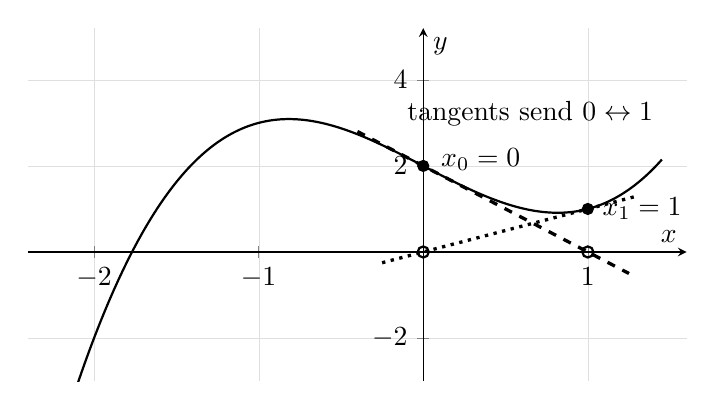
\begin{tikzpicture}
\begin{axis}[
    width=0.82\textwidth,
    height=0.50\textwidth,
    xmin=-2.4, xmax=1.6,
    ymin=-3.0, ymax=5.2,
    axis lines=middle,
    xlabel={\(x\)},
    ylabel={\(y\)},
    xtick={-2,-1,0,1},
    ytick={-2,0,2,4},
    grid=both,
    grid style={line width=.1pt, draw=gray!25},
]
\addplot[thick, domain=-2.25:1.45, samples=250] {x^3-2*x+2};
% Tangent at x=0: y=2-2x
\addplot[very thick, dashed, domain=-0.4:1.25, samples=2] {2-2*x};
% Tangent at x=1: y=x
\addplot[very thick, dotted, domain=-0.25:1.3, samples=2] {x};
\addplot[only marks, mark=*] coordinates {(0,2) (1,1)};
\addplot[only marks, mark=o, thick] coordinates {(1,0) (0,0)};
\node[anchor=west] at (axis cs:0.05,2.15) {\(x_0=0\)};
\node[anchor=west] at (axis cs:1.03,1.0) {\(x_1=1\)};
\node[anchor=south] at (axis cs:0.65,2.7) {tangents send \(0\leftrightarrow1\)};
\end{axis}
\end{tikzpicture}
\caption{For \(f(x)=x^3-2x+2\), Newton's method starting at \(0\) cycles between \(0\) and \(1\).}
\label{fig:newton-cycle}
\end{figure}

\paragraph{Failure mode 3: a multiple root.}
If a root \(r\) satisfies

\[
f'(r)=0,
\]

then Newton's method may still converge, but often more slowly.

For example,

\[
f(x)=(x-1)^2
\]

has a double root at

\[
x=1.
\]

Newton's method gives

\[
x_{n+1}
=
x_n-\frac{(x_n-1)^2}{2(x_n-1)}
=
x_n-\frac{x_n-1}{2}
=
\frac{x_n+1}{2},
\]

as long as \(x_n\neq1\).

This moves halfway toward \(1\) each time.  It converges, but the error is cut in
half rather than squared.  The fast convergence is lost.

\subsection{How to use Newton's method safely}
\label{subsec:using-newton-safely}

Newton's method is most reliable when it is used with a picture or with a bracket.

A practical workflow is:

\[
\begin{array}{ll}
\text{1.} & \text{Graph \(f\), or use signs to locate an interval where a root should lie.}\\
\text{2.} & \text{Choose a starting point near the root.}\\
\text{3.} & \text{Compute } x_{n+1}=x_n-\dfrac{f(x_n)}{f'(x_n)}.\\[10pt]
\text{4.} & \text{Stop only when both \(x_n\) has stabilized and \(f(x_n)\) is small.}\\
\text{5.} & \text{If the method behaves strangely, try a different starting point or use bisection.}
\end{array}
\]

The bisection method is slower, but if \(f\) is continuous and changes sign on an
interval, bisection is dependable.  Newton's method is faster when it behaves well.

\begin{quote}
\textbf{Newton's method in one sentence.}

Replace the curve by its tangent line, solve the linear problem, and repeat.
\end{quote}

Linear approximation has now done two jobs.  It estimated how errors move through
a formula, and it solved equations by tangent-line correction.

The next models take one more step.  Sometimes the rule we know is not a formula
for \(y\), but a formula for \(y'\).  Growth, decay, cooling, and population change are
often written first as laws about derivatives.
\section{Exponential growth and decay}
\label{sec:exponential-growth-decay}

Newton's method used a tangent line to solve an equation.  Linear approximation
helped us decide how far to move.

But many models do not first give an equation like

\[
f(x)=0.
\]

They give a law about change.

A population grows because each individual helps create more individuals.  A
radioactive substance decays because each atom has a chance to decay.  A bank
account grows because interest is earned on the current balance.  In each case, the
rate of change is tied to the amount already present.

That leads to the simplest and most important differential equation:

\[
y'=ky.
\]

\subsection{The differential equation \(y'=ky\)}
\label{subsec:differential-equation-y-prime-ky}

A \emph{differential equation} is an equation involving an unknown function and one
or more of its derivatives.

For example,

\[
y'=ky
\]

does not ask for a number \(y\).  It asks for a function \(y(t)\) whose derivative is
always \(k\) times the function itself.

The constant \(k\) controls the model.

\[
\begin{array}{c|c}
\textbf{sign of }k & \textbf{meaning} \\ \hline
k>0 & \text{growth} \\
k=0 & \text{no change} \\
k<0 & \text{decay}
\end{array}
\]

The units of \(k\) are important.  If \(y\) is measured in grams and \(t\) in years, then

\[
y'
\]

has units

\[
\text{grams/year}.
\]

So in

\[
y'=ky,
\]

the constant \(k\) must have units

\[
\frac{1}{\text{year}}.
\]

It is a relative rate of change.

\paragraph{Example: a first growth model.}
Suppose a small bacterial culture satisfies

\[
P'(t)=0.4P(t),
\]

where \(t\) is measured in hours.  If

\[
P(0)=500,
\]

find \(P(t)\).

The equation says that the population grows at a rate equal to \(40\%\) of its current
size per hour.  We need a function whose derivative is \(0.4\) times the function.

Since

\[
\frac{d}{dt}e^{0.4t}=0.4e^{0.4t},
\]

a natural solution is

\[
P(t)=Ce^{0.4t}.
\]

Use the initial condition:

\[
P(0)=Ce^0=C.
\]

Since \(P(0)=500\),

\[
C=500.
\]

Therefore

\[
\boxed{
P(t)=500e^{0.4t}.
}
\]

The population grows exponentially.

\begin{figure}[h]
\centering
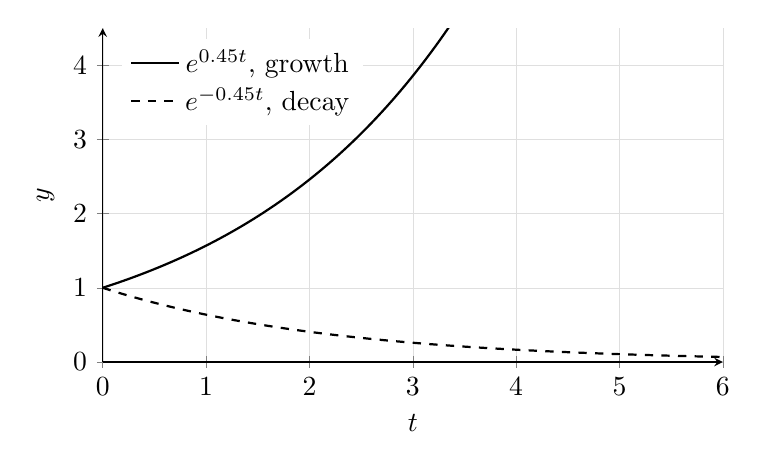
\begin{tikzpicture}
\begin{axis}[
    width=0.78\textwidth,
    height=0.48\textwidth,
    xmin=0, xmax=6,
    ymin=0, ymax=4.5,
    axis lines=left,
    xlabel={\(t\)},
    ylabel={\(y\)},
    xtick={0,1,2,3,4,5,6},
    ytick={0,1,2,3,4},
    grid=both,
    grid style={line width=.1pt, draw=gray!25},
    legend style={draw=none, at={(0.03,0.97)}, anchor=north west}
]
\addplot[thick, domain=0:6, samples=150] {exp(0.45*x)};
\addlegendentry{\(e^{0.45t}\), growth}
\addplot[thick, dashed, domain=0:6, samples=150] {exp(-0.45*x)};
\addlegendentry{\(e^{-0.45t}\), decay}
\end{axis}
\end{tikzpicture}
\caption{The equation \(y'=ky\) gives exponential growth when \(k>0\) and exponential decay when \(k<0\).}
\label{fig:exponential-growth-decay}
\end{figure}

The example gives the general pattern.

\begin{quote}
\textbf{Exponential growth and decay equation.}
If

\[
y'=ky
\]

and

\[
y(0)=y_0,
\]

then

\[
\boxed{
y(t)=y_0e^{kt}.
}
\]
\end{quote}

\paragraph{Proof.}
Suppose \(y\) satisfies

\[
y'=ky.
\]

Multiply \(y(t)\) by \(e^{-kt}\).  Let

\[
u(t)=e^{-kt}y(t).
\]

Then, by the product rule,

\[
u'(t)
=
(-k)e^{-kt}y(t)+e^{-kt}y'(t).
\]

Factor:

\[
u'(t)=e^{-kt}\bigl(y'(t)-ky(t)\bigr).
\]

Since \(y'=ky\), we get

\[
u'(t)=0.
\]

So \(u(t)\) is constant.  Therefore

\[
e^{-kt}y(t)=C,
\]

and hence

\[
y(t)=Ce^{kt}.
\]

Using \(y(0)=y_0\),

\[
y_0=Ce^0=C.
\]

So

\[
y(t)=y_0e^{kt}.
\]

This proves the formula.

\begin{quote}
\textbf{Meaning of the equation.}

\[
y'=ky
\]

is equivalent to

\[
\frac{y'}{y}=k
\]

when \(y\neq0\).  The relative rate of change is constant.  That is the defining
feature of exponential growth and decay.
\end{quote}

\subsection{Half-life and doubling time}
\label{subsec:half-life-doubling-time}

The constant \(k\) is not always the most natural way to describe exponential change.

For growth, we often describe a quantity by its \emph{doubling time}: the time it takes
to multiply by \(2\).

For decay, we often describe a quantity by its \emph{half-life}: the time it takes to
multiply by \(1/2\).

Suppose

\[
y(t)=y_0e^{kt}.
\]

If \(k>0\), the doubling time \(D\) satisfies

\[
y(D)=2y_0.
\]

So

\[
y_0e^{kD}=2y_0.
\]

Assuming \(y_0\neq0\),

\[
e^{kD}=2.
\]

Take natural logarithms:

\[
kD=\ln 2.
\]

Therefore

\[
\boxed{
D=\frac{\ln2}{k}.
}
\]

For decay, \(k<0\).  The half-life \(H\) satisfies

\[
y(H)=\frac12y_0.
\]

So

\[
y_0e^{kH}=\frac12y_0.
\]

Thus

\[
e^{kH}=\frac12.
\]

Taking logarithms,

\[
kH=\ln\left(\frac12\right)=-\ln2.
\]

Therefore

\[
\boxed{
H=-\frac{\ln2}{k}
}
\]

when \(k<0\).

\paragraph{Example: decay from a half-life.}
A substance has half-life \(6\) hours.  If the initial amount is \(A_0\), find the amount
after \(24\) hours.

Since \(24\) hours is

\[
\frac{24}{6}=4
\]

half-lives, the amount is multiplied by \(1/2\) four times:

\[
A(24)=A_0\left(\frac12\right)^4.
\]

Thus

\[
\boxed{
A(24)=\frac{A_0}{16}.
}
\]

Using the exponential formula, half-life \(H=6\) gives

\[
k=-\frac{\ln2}{6}.
\]

So

\[
A(t)=A_0e^{-(\ln2)t/6}.
\]

This can also be written as

\[
A(t)=A_0\left(\frac12\right)^{t/6}.
\]

That form makes the half-life visible.

\begin{quote}
\textbf{Half-life form.}
If a quantity has half-life \(H\), then

\[
\boxed{
A(t)=A_0\left(\frac12\right)^{t/H}.
}
\]
\end{quote}

\begin{quote}
\textbf{Doubling-time form.}
If a quantity has doubling time \(D\), then

\[
\boxed{
A(t)=A_0\,2^{t/D}.
}
\]
\end{quote}

These are the same exponential model written in a way that matches the information
given.

\paragraph{Example: estimating a doubling time.}
A population grows according to

\[
P'(t)=0.03P(t),
\]

where \(t\) is measured in years.  Its doubling time is

\[
D=\frac{\ln2}{0.03}.
\]

Since

\[
\ln2\approx0.693,
\]

we get

\[
D\approx\frac{0.693}{0.03}\approx23.1.
\]

The population doubles in about \(23.1\) years.

\subsection{Continuously compounded interest}
\label{subsec:continuously-compounded-interest}

Money in an account can also be modeled by

\[
A'=rA.
\]

Here

\[
A(t)
\]

is the account balance after \(t\) years, and \(r\) is the annual interest rate written as a
decimal.

If

\[
r=0.05,
\]

then the account grows at \(5\%\) per year.  The continuously compounded model is

\[
A'=0.05A.
\]

So

\[
\boxed{
A(t)=A_0e^{0.05t}.
}
\]

More generally, if the initial deposit is \(P\), then

\[
\boxed{
A(t)=Pe^{rt}.
}
\]

\paragraph{Example.}
Suppose \(1000\) dollars is invested at \(5\%\) annual interest, compounded
continuously.  Find the value after \(10\) years.

The model is

\[
A(t)=1000e^{0.05t}.
\]

Thus

\[
A(10)=1000e^{0.5}.
\]

Since

\[
e^{0.5}\approx1.64872,
\]

we get

\[
\boxed{
A(10)\approx1648.72
}
\]

dollars.

\begin{quote}
\textbf{Interest as a rate law.}

Continuous compounding means that interest is earned on the current balance at every
instant:

\[
A'=rA.
\]

That rate law forces the exponential formula

\[
A(t)=Pe^{rt}.
\]
\end{quote}

There is a useful connection with ordinary compounding.  If interest is compounded
\(n\) times per year, then

\[
A_n(t)=P\left(1+\frac{r}{n}\right)^{nt}.
\]

As \(n\) gets larger, this approaches

\[
Pe^{rt}.
\]

So continuous compounding is the limiting case of more and more frequent
compounding.

\subsection{Newton's law of cooling}
\label{subsec:newtons-law-cooling}

Not every exponential model has the form

\[
T'=kT.
\]

A hot cup of coffee in a room does not cool toward \(0^\circ\).  It cools toward the
room temperature.

The natural changing quantity is not the temperature \(T\) itself, but the temperature
difference between the coffee and the room.

Let

\[
T(t)=\text{temperature of the object at time }t,
\]

and let

\[
T_s=\text{surrounding temperature}.
\]

Newton's law of cooling says:

\[
\boxed{
T'=-k(T-T_s),
\qquad k>0.
}
\]

The difference

\[
T-T_s
\]

decays exponentially.

Let

\[
D(t)=T(t)-T_s.
\]

Since \(T_s\) is constant,

\[
D'(t)=T'(t).
\]

The cooling law becomes

\[
D'=-kD.
\]

Therefore

\[
D(t)=D(0)e^{-kt}.
\]

Since

\[
D(0)=T(0)-T_s,
\]

we get

\[
\boxed{
T(t)=T_s+\bigl(T(0)-T_s\bigr)e^{-kt}.
}
\]

\paragraph{Example: cooling coffee.}
A cup of coffee is \(90^\circ\text{C}\) when placed in a room whose temperature is

\[
20^\circ\text{C}.
\]

After \(10\) minutes, the coffee is

\[
60^\circ\text{C}.
\]

Assuming Newton's law of cooling, estimate the temperature after \(30\) minutes.

The model is

\[
T(t)=20+(90-20)e^{-kt}.
\]

So

\[
T(t)=20+70e^{-kt}.
\]

Use \(T(10)=60\):

\[
60=20+70e^{-10k}.
\]

Then

\[
40=70e^{-10k},
\]

so

\[
e^{-10k}=\frac{4}{7}.
\]

Thus

\[
k=\frac{1}{10}\ln\left(\frac74\right).
\]

Now find \(T(30)\).  Since

\[
e^{-10k}=\frac47,
\]

we have

\[
e^{-30k}=\left(e^{-10k}\right)^3=\left(\frac47\right)^3.
\]

Therefore

\[
T(30)=20+70\left(\frac47\right)^3.
\]

Compute:

\[
\left(\frac47\right)^3=\frac{64}{343}.
\]

So

\[
T(30)=20+70\cdot\frac{64}{343}
=
20+\frac{4480}{343}.
\]

Thus

\[
\boxed{
T(30)\approx33.1^\circ\text{C}.
}
\]

\begin{figure}[h]
\centering
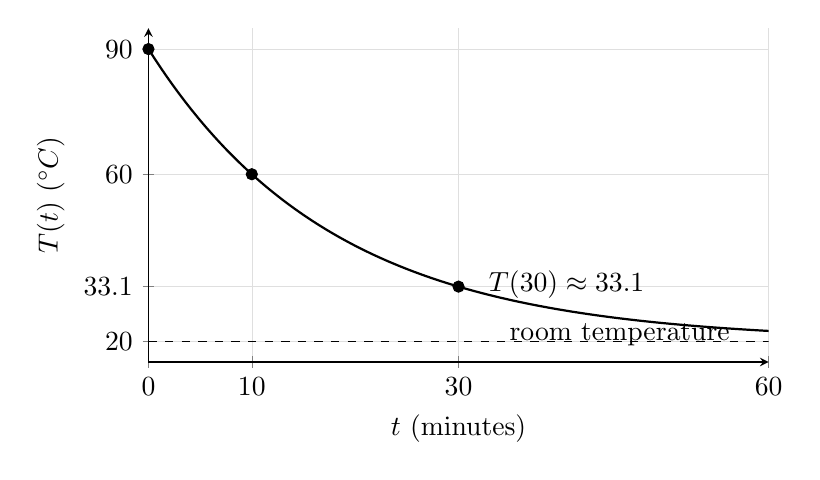
\begin{tikzpicture}
\begin{axis}[
    width=0.78\textwidth,
    height=0.48\textwidth,
    xmin=0, xmax=60,
    ymin=15, ymax=95,
    axis lines=left,
    xlabel={\(t\) (minutes)},
    ylabel={\(T(t)\) (\(^\circ\text{C}\))},
    xtick={0,10,30,60},
    ytick={20,33.1,60,90},
    grid=both,
    grid style={line width=.1pt, draw=gray!25},
]
\addplot[thick, domain=0:60, samples=200] {20+70*exp(-0.05596*x)};
\addplot[dashed, domain=0:60, samples=2] {20};
\addplot[only marks, mark=*] coordinates {(0,90) (10,60) (30,33.06)};
\node[anchor=west] at (axis cs:32,33.5) {\(T(30)\approx33.1\)};
\node[anchor=west] at (axis cs:34,21.5) {room temperature};
\end{axis}
\end{tikzpicture}
\caption{Newton's law of cooling says the temperature difference \(T-T_s\) decays exponentially.}
\label{fig:newton-cooling-coffee}
\end{figure}

\subsection{What exponential models assume}
\label{subsec:what-exponential-models-assume}

Exponential models are powerful because they are simple.  Their simplicity is also
their danger.

The equation

\[
y'=ky
\]

says that the relative rate of change is constant:

\[
\frac{y'}{y}=k.
\]

If that ratio is not constant, the model is not exponential.

\paragraph{Warning example.}
Let

\[
y(t)=100+t^2.
\]

Then

\[
y'(t)=2t.
\]

The quantity is increasing for \(t>0\), but it is not growing exponentially.  Its relative
rate of change is

\[
\frac{y'(t)}{y(t)}
=
\frac{2t}{100+t^2}.
\]

This depends on \(t\).  It is not constant.

So increasing does not mean exponential.  Even fast increasing does not mean
exponential.  Exponential growth means constant relative growth.

\begin{quote}
\textbf{How to recognize the exponential model.}

A quantity is modeled by

\[
y'=ky
\]

when its rate of change is proportional to its current amount.

Equivalently, when \(y\neq0\),

\[
\frac{y'}{y}=k
\]

is constant.
\end{quote}

Exponential growth is often a good first approximation.  But it cannot continue
forever in a world with limited space, food, money, or people.  The next model keeps
the early exponential behavior but builds in a ceiling.

\section{Logistic growth and limited resources}
\label{sec:logistic-growth-limited-resources}

Exponential growth has no memory of limits.  If

\[
P'=rP,
\]

then a positive population keeps growing faster and faster forever.

That can describe the beginning of a process.  It cannot describe the whole life of a
population in a bounded environment.  A petri dish has limited nutrients.  A lake has
limited space.  A rumor has only so many people left to reach.

The first correction is simple:

\[
\text{growth should slow down as the quantity approaches a maximum size.}
\]

That idea leads to the logistic equation.

\subsection{Why pure exponential growth cannot last}
\label{subsec:why-exponential-growth-cannot-last}

Suppose a population doubles every hour.  If it starts with \(100\) individuals, then
after \(n\) hours it has size

\[
100\cdot2^n.
\]

After \(10\) hours,

\[
100\cdot2^{10}=102{,}400.
\]

After \(20\) hours,

\[
100\cdot2^{20}=104{,}857{,}600.
\]

After \(40\) hours,

\[
100\cdot2^{40}
\]

is enormous.

The problem is not that the early exponential model is useless.  It may be excellent
at the beginning.  The problem is that the model has no built-in stopping mechanism.

If the environment can support at most \(K\) individuals, then the growth rate should
be large when \(P\) is small and close to \(0\) when \(P\) is near \(K\).

The simplest factor with that behavior is

\[
1-\frac{P}{K}.
\]

When \(P\) is small compared with \(K\), this factor is close to \(1\).  The model looks
almost exponential.

When \(P=K\), the factor becomes

\[
1-\frac{K}{K}=0.
\]

Growth stops.

\subsection{The logistic differential equation}
\label{subsec:logistic-differential-equation}

The logistic model is

\[
\boxed{
P'=rP\left(1-\frac{P}{K}\right),
\qquad r>0,\quad K>0.
}
\]

Here

\[
P(t)=\text{population at time }t,
\]

\[
r=\text{early relative growth rate},
\]

and

\[
K=\text{carrying capacity}.
\]

The carrying capacity is the level the environment can support in the model.

The equation contains two factors:

\[
rP
\]

and

\[
1-\frac{P}{K}.
\]

The first factor says that more individuals create more possible growth.  The second
factor says that limited resources reduce growth as \(P\) approaches \(K\).

\[
\begin{array}{c|c|c}
\textbf{population size} & 1-\dfrac{P}{K} & \textbf{model behavior} \\ \hline
P\ll K & \approx1 & P'\approx rP,\ \text{almost exponential} \\[6pt]
P=K/2 & 1/2 & \text{growth still positive} \\[6pt]
P=K & 0 & \text{growth stops} \\[6pt]
P>K & <0 & \text{population decreases}
\end{array}
\]

\begin{quote}
\textbf{Logistic growth.}

The logistic equation

\[
P'=rP\left(1-\frac{P}{K}\right)
\]

keeps the early exponential behavior \(P'\approx rP\), but slows the growth as
\(P\) approaches the carrying capacity \(K\).
\end{quote}

\subsection{Equilibria and stability from a graph}
\label{subsec:equilibria-stability-graph}

A solution is in equilibrium if it does not change.  That means

\[
P'=0.
\]

For the logistic equation,

\[
P'=rP\left(1-\frac{P}{K}\right).
\]

So

\[
P'=0
\]

when

\[
P=0
\]

or

\[
1-\frac{P}{K}=0.
\]

Thus the equilibrium levels are

\[
\boxed{
P=0
\qquad\text{and}\qquad
P=K.
}
\]

The sign of \(P'\) tells how solutions move.

If

\[
0<P<K,
\]

then

\[
P>0
\qquad\text{and}\qquad
1-\frac{P}{K}>0,
\]

so

\[
P'>0.
\]

The population increases.

If

\[
P>K,
\]

then

\[
1-\frac{P}{K}<0,
\]

so

\[
P'<0.
\]

The population decreases.

Therefore \(P=K\) is stable: populations below \(K\) move upward, and populations
above \(K\) move downward.

The equilibrium \(P=0\) is unstable on the physical side.  If the population is just
above \(0\), it grows away from \(0\).

\begin{figure}[h]
\centering
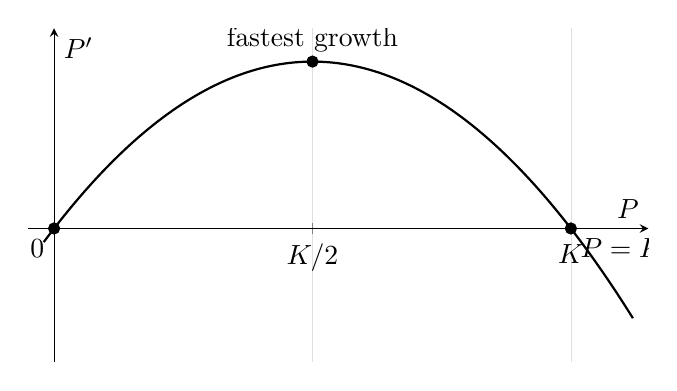
\begin{tikzpicture}
\begin{axis}[
    width=0.78\textwidth,
    height=0.48\textwidth,
    xmin=-0.5, xmax=11.5,
    ymin=-1.2, ymax=1.8,
    axis lines=middle,
    xlabel={\(P\)},
    ylabel={\(P'\)},
    xtick={0,5,10},
    xticklabels={\(0\),\(K/2\),\(K\)},
    ytick={0},
    grid=both,
    grid style={line width=.1pt, draw=gray!25},
]
\addplot[thick, domain=-0.2:11.2, samples=200] {0.6*x*(1-x/10)};
\addplot[only marks, mark=*] coordinates {(0,0) (10,0) (5,1.5)};
\node[anchor=south] at (axis cs:5,1.5) {fastest growth};
\node[anchor=north east] at (axis cs:0,0) {\(P=0\)};
\node[anchor=north west] at (axis cs:10,0) {\(P=K\)};
\end{axis}
\end{tikzpicture}

\vspace{0.8em}

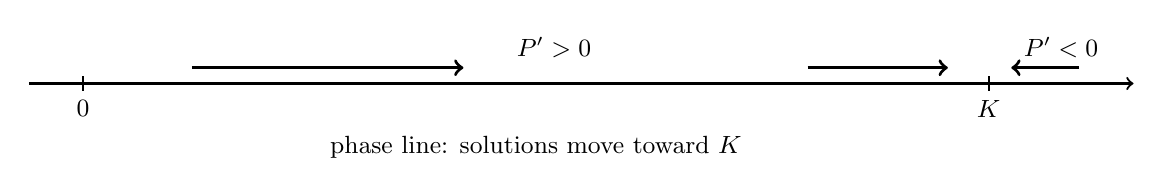
\begin{tikzpicture}[xscale=1.15, every node/.style={font=\small}]
  \draw[->, thick] (-0.6,0) -- (11.6,0);
  \foreach \x/\lab in {0/\(0\),10/\(K\)} {
    \draw[thick] (\x,0.09) -- (\x,-0.09);
    \node[below] at (\x,-0.09) {\lab};
  }
  \draw[->, very thick] (1.2,0.2) -- (4.2,0.2);
  \draw[->, very thick] (8.0,0.2) -- (9.55,0.2);
  \draw[->, very thick] (11.0,0.2) -- (10.25,0.2);
  \node[above] at (5.2,0.2) {\(P'>0\)};
  \node[above] at (10.8,0.2) {\(P'<0\)};
  \node[below] at (5,-0.55) {phase line: solutions move toward \(K\)};
\end{tikzpicture}

\caption{For the logistic equation, \(P'\) is positive below \(K\) and negative above \(K\).  The carrying capacity \(K\) is stable.}
\label{fig:logistic-phase-line}
\end{figure}

There is another important point in the graph of

\[
P'=rP\left(1-\frac{P}{K}\right).
\]

As a function of \(P\), the right side is a downward-opening parabola.  It reaches its
maximum at

\[
P=\frac{K}{2}.
\]

So logistic growth is fastest when the population is halfway to the carrying capacity.

\[
\boxed{
\text{In the logistic model, the fastest growth occurs at }P=K/2.
}
\]

\subsection{The logistic formula}
\label{subsec:logistic-formula}

The logistic equation can be solved using a clever change of variables.  The idea is to
measure how much room remains compared with the current population.

Assume

\[
P(t)>0.
\]

Define

\[
Q(t)=\frac{K}{P(t)}-1.
\]

This quantity is positive when \(0<P<K\).  It measures the remaining room relative
to the population.

Differentiate:

\[
Q'(t)
=
-K\frac{P'(t)}{P(t)^2}.
\]

Using the logistic equation,

\[
P'=rP\left(1-\frac{P}{K}\right),
\]

we get

\[
Q'
=
-K\frac{rP\left(1-\frac{P}{K}\right)}{P^2}.
\]

Simplify:

\[
Q'
=
-r\frac{K}{P}\left(1-\frac{P}{K}\right).
\]

Since

\[
\frac{K}{P}\left(1-\frac{P}{K}\right)
=
\frac{K}{P}-1
=
Q,
\]

we obtain

\[
Q'=-rQ.
\]

That is exponential decay.

Therefore

\[
Q(t)=Q(0)e^{-rt}.
\]

If

\[
P(0)=P_0>0,
\]

then

\[
Q(0)=\frac{K}{P_0}-1=\frac{K-P_0}{P_0}.
\]

Let

\[
A=\frac{K-P_0}{P_0}.
\]

Then

\[
\frac{K}{P(t)}-1=Ae^{-rt}.
\]

So

\[
\frac{K}{P(t)}=1+Ae^{-rt}.
\]

Finally,

\[
\boxed{
P(t)=\frac{K}{1+Ae^{-rt}},
\qquad
A=\frac{K-P_0}{P_0}.
}
\]

This is the logistic formula.

\begin{quote}
\textbf{Logistic solution with positive initial population.}
If

\[
P'=rP\left(1-\frac{P}{K}\right),
\qquad
P(0)=P_0>0,
\]

then

\[
\boxed{
P(t)=\frac{K}{1+\left(\dfrac{K-P_0}{P_0}\right)e^{-rt}}.
}
\]
\end{quote}

The formula also shows the long-term behavior.  Since

\[
e^{-rt}\to0
\qquad\text{as}\qquad t\to\infty,
\]

we get

\[
P(t)\to\frac{K}{1+0}=K.
\]

So the population approaches the carrying capacity.

\paragraph{The missing equilibrium \(P=0\).}
The formula above assumed

\[
P_0>0,
\]

because we divided by \(P\).  The initial value

\[
P_0=0
\]

is a separate equilibrium solution:

\[
P(t)=0.
\]

If there is no population, the logistic model creates no population from nothing.

\paragraph{Example: reaching half the carrying capacity.}
A population satisfies

\[
P'=0.8P\left(1-\frac{P}{1000}\right),
\qquad
P(0)=100.
\]

Here

\[
r=0.8,
\qquad
K=1000,
\qquad
P_0=100.
\]

So

\[
A=\frac{1000-100}{100}=9.
\]

The solution is

\[
P(t)=\frac{1000}{1+9e^{-0.8t}}.
\]

When does the population reach \(500\), half the carrying capacity?

Set

\[
500=\frac{1000}{1+9e^{-0.8t}}.
\]

Then

\[
1+9e^{-0.8t}=2.
\]

So

\[
9e^{-0.8t}=1,
\]

hence

\[
e^{-0.8t}=\frac19.
\]

Taking logarithms,

\[
-0.8t=-\ln9.
\]

Therefore

\[
t=\frac{\ln9}{0.8}.
\]

Since

\[
\ln9\approx2.197,
\]

we get

\[
\boxed{
t\approx2.75.
}
\]

The population reaches \(500\) after about \(2.75\) time units.

\begin{figure}[h]
\centering
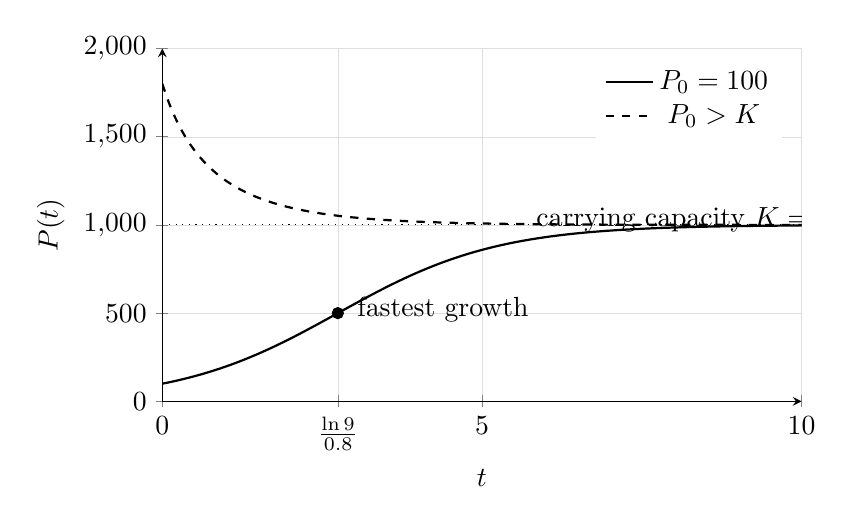
\begin{tikzpicture}
\begin{axis}[
    width=0.80\textwidth,
    height=0.50\textwidth,
    xmin=0, xmax=10,
    ymin=0, ymax=2000,
    axis lines=left,
    xlabel={\(t\)},
    ylabel={\(P(t)\)},
    xtick={0,2.75,5,10},
    xticklabels={\(0\),\(\frac{\ln9}{0.8}\),\(5\),\(10\)},
    ytick={0,500,1000,1500,2000},
    grid=both,
    grid style={line width=.1pt, draw=gray!25},
    legend style={draw=none, at={(0.97,0.97)}, anchor=north east}
]
\addplot[thick, domain=0:10, samples=200] {1000/(1+9*exp(-0.8*x))};
\addlegendentry{\(P_0=100\)}
\addplot[thick, dashed, domain=0:10, samples=200] {1000/(1-0.444444*exp(-0.8*x))};
\addlegendentry{\(P_0>K\)}
\addplot[dotted, domain=0:10, samples=2] {1000};
\addplot[only marks, mark=*] coordinates {(2.746,500)};
\node[anchor=west] at (axis cs:5.7,1030) {carrying capacity \(K=1000\)};
\node[anchor=west] at (axis cs:2.9,520) {fastest growth};
\end{axis}
\end{tikzpicture}
\caption{Logistic solutions move toward the carrying capacity \(K\).  From below they rise toward \(K\); from above they fall toward \(K\).}
\label{fig:logistic-solutions}
\end{figure}

\subsection{Population and spread models}
\label{subsec:population-spread-models}

The logistic equation appears whenever two ideas are both reasonable:

\[
\text{more current amount creates more growth}
\]

and

\[
\text{limited remaining capacity slows growth}.
\]

For populations, the current amount is the population \(P\), and the limiting factor is
the carrying capacity \(K\).

For a rumor, the current amount may be the number of people who have heard it.  The
limiting factor is the number of people who have not yet heard it.

Suppose a school has

\[
K=2000
\]

students, and \(R(t)\) is the number who have heard a rumor after \(t\) days.  A simple
logistic model is

\[
R'=0.7R\left(1-\frac{R}{2000}\right).
\]

If

\[
R(0)=20,
\]

then

\[
A=\frac{2000-20}{20}=99.
\]

So

\[
R(t)=\frac{2000}{1+99e^{-0.7t}}.
\]

The rumor spreads slowly at first because few people know it.  It then spreads quickly
when many people know it and many people remain to hear it.  Finally it slows again
because most people have already heard it.

This slow--fast--slow shape is the signature of a logistic curve.

\begin{quote}
\textbf{The logistic story.}

\[
\begin{array}{c|c}
\textbf{early stage} & P\ll K,\quad P'\approx rP,\quad \text{almost exponential} \\[4pt]
\textbf{middle stage} & P\approx K/2,\quad \text{growth is fastest} \\[4pt]
\textbf{late stage} & P\approx K,\quad P'\approx0,\quad \text{growth slows}
\end{array}
\]
\end{quote}

\subsection{What logistic models assume}
\label{subsec:what-logistic-models-assume}

The logistic model is more realistic than pure exponential growth, but it is still a
model.

It assumes:

\[
\begin{array}{ll}
\text{1.} & \text{the carrying capacity \(K\) is fixed,}\\
\text{2.} & \text{the early growth rate \(r\) is fixed,}\\
\text{3.} & \text{the slowing factor is linear in \(P\),}\\
\text{4.} & \text{there are no delays, shocks, seasons, migrations, or changing behavior.}
\end{array}
\]

Those assumptions may be useful, but they are not automatic.

\paragraph{Warning example: early data can be misleading.}
When

\[
P\ll K,
\]

the logistic equation

\[
P'=rP\left(1-\frac{P}{K}\right)
\]

looks like

\[
P'\approx rP.
\]

So early logistic growth and exponential growth can look almost the same.

That means early data may reveal \(r\), but it may not reveal \(K\).  To estimate the
carrying capacity, we need data from the stage where growth begins to slow.

\begin{quote}
\textbf{A model is a promise with conditions.}

Exponential growth promises constant relative growth.

Logistic growth promises constant early relative growth and a fixed carrying capacity.

Before trusting the formula, check whether the promise matches the situation.
\end{quote}

This chapter used derivatives to answer practical questions: rates related to rates,
best choices, local approximations, root finding, and models whose laws are written
as differential equations.

But we have postponed the other half of calculus.  If a derivative tells how fast
something changes, how do we recover the total change?  If velocity is known at every
instant, how do we rebuild distance?

That question leads back to the first chapter, where area under a velocity graph was
waiting for us.  The next chapter begins the integral.
\section{Light, time, and extremal principles}
\label{sec:light-time-extremal-principles}

Optimization problems usually begin with an ordinary choice: a width, a height, a
price, a radius, a time.  The derivative helps us find the best value of that choice.

But some of the most beautiful optimization problems ask for more than a number.
They ask for a path.

Light gives the simplest surprise.  A ray of light reflecting from a mirror behaves as
if it has solved an optimization problem.  A ray passing from air into water behaves as
if it has solved a different one.

The calculus is the same calculus we have been using:

\[
\text{write the quantity to be minimized, differentiate, set the derivative equal to }0.
\]

The meaning is deeper.  A law of nature can sometimes be written as a best-choice
principle.

\subsection{Reflection from shortest path}
\label{subsec:reflection-shortest-path}

Suppose a light ray travels from a point \(A\) to a mirror and then to a point \(B\).
Where should it strike the mirror?

Place the mirror on the \(x\)-axis.  Let

\[
A=(0,a),
\qquad
B=(L,b),
\]

where

\[
a>0,\qquad b>0,\qquad L>0.
\]

Let the reflection point be

\[
P=(x,0),
\qquad 0\le x\le L.
\]

The total path length is

\[
D(x)=\sqrt{x^2+a^2}+\sqrt{(L-x)^2+b^2}.
\]

The first term is the distance from \(A\) to \(P\).  The second term is the distance
from \(P\) to \(B\).

Differentiate:

\[
D'(x)
=
\frac{x}{\sqrt{x^2+a^2}}
-
\frac{L-x}{\sqrt{(L-x)^2+b^2}}.
\]

At a shortest interior path, we must have

\[
D'(x)=0.
\]

Thus

\[
\frac{x}{\sqrt{x^2+a^2}}
=
\frac{L-x}{\sqrt{(L-x)^2+b^2}}.
\]

Now interpret the two fractions geometrically.

Let \(\alpha\) be the angle that the incoming ray makes with the normal to the
mirror.  Let \(\beta\) be the angle that the outgoing ray makes with the normal.
Then

\[
\sin\alpha=\frac{x}{\sqrt{x^2+a^2}},
\]

and

\[
\sin\beta=\frac{L-x}{\sqrt{(L-x)^2+b^2}}.
\]

So the critical-point equation becomes

\[
\sin\alpha=\sin\beta.
\]

Since both angles lie between \(0\) and \(\pi/2\), this gives

\[
\boxed{\alpha=\beta.}
\]

The angle of incidence equals the angle of reflection.

\begin{figure}[h]
\centering
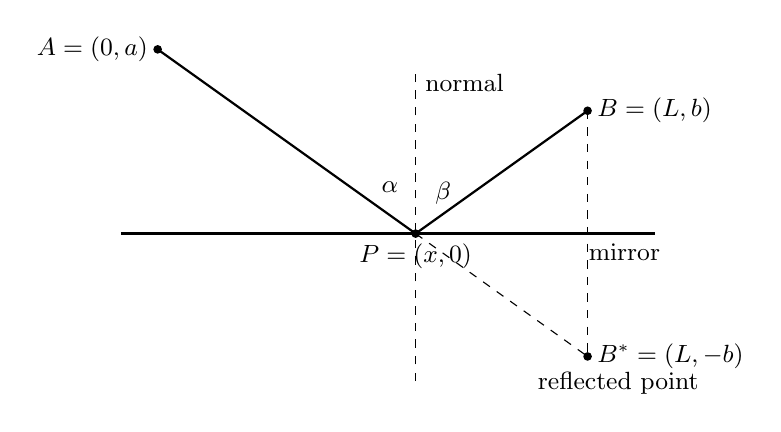
\begin{tikzpicture}[scale=0.78, every node/.style={font=\small}]
  % mirror
  \draw[very thick] (-0.6,0) -- (8.1,0);
  \node[below] at (7.6,0) {mirror};

  % coordinates
  \coordinate (A) at (0,3);
  \coordinate (P) at (4.2,0);
  \coordinate (B) at (7,2);
  \coordinate (Bstar) at (7,-2);

  % paths
  \draw[thick] (A) -- (P) -- (B);
  \draw[dashed] (P) -- (Bstar);
  \draw[dashed] (B) -- (Bstar);

  % normal
  \draw[dashed] (4.2,-2.4) -- (4.2,2.6);
  \node[right] at (4.2,2.45) {normal};

  % points
  \fill (A) circle (2pt);
  \fill (P) circle (2pt);
  \fill (B) circle (2pt);
  \fill (Bstar) circle (2pt);

  \node[left] at (A) {\(A=(0,a)\)};
  \node[below] at (P) {\(P=(x,0)\)};
  \node[right] at (B) {\(B=(L,b)\)};
  \node[right] at (Bstar) {\(B^*=(L,-b)\)};

  % angle labels, approximate
  \node at (3.78,0.75) {\(\alpha\)};
  \node at (4.65,0.65) {\(\beta\)};

  % reflected line label
  \node[below] at (7.5,-2.1) {reflected point};
\end{tikzpicture}
\caption{Reflecting \(B\) across the mirror turns the broken reflected path into a straight path from \(A\) to \(B^*\).}
\label{fig:reflection-reflected-point}
\end{figure}

There is also a geometric shortcut.  Reflect \(B\) across the mirror to

\[
B^*=(L,-b).
\]

The broken path

\[
A\to P\to B
\]

has the same length as the straightened path

\[
A\to P\to B^*.
\]

The shortest path from \(A\) to \(B^*\) is a straight line.  So the best \(P\) is where
that straight line crosses the mirror.

The derivative and the geometry say the same thing.

\begin{quote}
\textbf{Law of reflection.}

A reflected light ray makes equal angles with the normal:

\[
\boxed{
\text{angle of incidence}=\text{angle of reflection}.
}
\]
\end{quote}

The second derivative confirms that the critical point is a minimum:

\[
D''(x)
=
\frac{a^2}{(x^2+a^2)^{3/2}}
+
\frac{b^2}{((L-x)^2+b^2)^{3/2}}
>0.
\]

So \(D\) is concave up on the interval.  The stationary point is the shortest path.

\subsection{Refraction and Snell's law}
\label{subsec:refraction-snells-law}

Reflection minimizes distance because the light stays in one medium.  Refraction is
different.

When light passes from one medium into another, its speed changes.  The best path is
not the shortest path.  It is the path of least time.

Suppose the upper medium has speed \(v_1\), and the lower medium has speed \(v_2\).
Let the boundary between the two media be the \(x\)-axis.  Place

\[
A=(0,a)
\]

above the boundary and

\[
B=(L,-b)
\]

below the boundary, where \(a,b,L>0\).  Let the crossing point be

\[
P=(x,0).
\]

The travel time is

\[
T(x)
=
\frac{\sqrt{x^2+a^2}}{v_1}
+
\frac{\sqrt{(L-x)^2+b^2}}{v_2}.
\]

Differentiate:

\[
T'(x)
=
\frac{x}{v_1\sqrt{x^2+a^2}}
-
\frac{L-x}{v_2\sqrt{(L-x)^2+b^2}}.
\]

At an interior minimum,

\[
T'(x)=0.
\]

Therefore

\[
\frac{x}{v_1\sqrt{x^2+a^2}}
=
\frac{L-x}{v_2\sqrt{(L-x)^2+b^2}}.
\]

Let \(\theta_1\) be the angle the upper ray makes with the normal, and let
\(\theta_2\) be the angle the lower ray makes with the normal.  Then

\[
\sin\theta_1=\frac{x}{\sqrt{x^2+a^2}},
\]

and

\[
\sin\theta_2=\frac{L-x}{\sqrt{(L-x)^2+b^2}}.
\]

So the minimizing condition becomes

\[
\boxed{
\frac{\sin\theta_1}{v_1}
=
\frac{\sin\theta_2}{v_2}.
}
\]

This is Snell's law in speed form.

If \(c\) is the speed of light in vacuum and

\[
n=\frac{c}{v}
\]

is the index of refraction, then

\[
v=\frac{c}{n}.
\]

Substituting into the speed form gives

\[
\frac{\sin\theta_1}{c/n_1}
=
\frac{\sin\theta_2}{c/n_2}.
\]

Cancel \(c\):

\[
n_1\sin\theta_1=n_2\sin\theta_2.
\]

So Snell's law is also written as

\[
\boxed{
n_1\sin\theta_1=n_2\sin\theta_2.
}
\]

\begin{figure}[h]
\centering
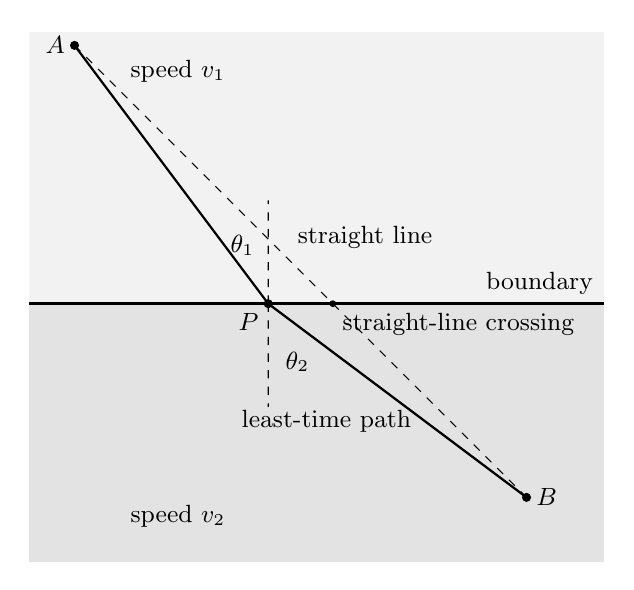
\begin{tikzpicture}[scale=0.82, every node/.style={font=\small}]
  % media shading
  \fill[gray!10] (-0.7,0) rectangle (8.2,4.2);
  \fill[gray!22] (-0.7,-4.0) rectangle (8.2,0);

  % boundary
  \draw[very thick] (-0.7,0) -- (8.2,0);
  \node[above] at (7.2,0) {boundary};

  % points
  \coordinate (A) at (0,4);
  \coordinate (P) at (3,0);
  \coordinate (B) at (7,-3);
  \coordinate (S) at (4,0);

  \draw[thick] (A) -- (P) -- (B);
  \draw[dashed] (A) -- (B);
  \draw[dashed] (P) -- (3,1.6);
  \draw[dashed] (P) -- (3,-1.6);

  \fill (A) circle (2pt);
  \fill (P) circle (2pt);
  \fill (B) circle (2pt);
  \fill (S) circle (1.5pt);

  \node[left] at (A) {\(A\)};
  \node[below left] at (P) {\(P\)};
  \node[right] at (B) {\(B\)};
  \node[below right] at (S) {straight-line crossing};

  \node at (1.6,3.6) {speed \(v_1\)};
  \node at (1.6,-3.3) {speed \(v_2\)};

  \node at (2.6,0.9) {\(\theta_1\)};
  \node at (3.45,-0.9) {\(\theta_2\)};

  \node[above] at (4.5,0.7) {straight line};
  \node[below] at (3.9,-1.5) {least-time path};
\end{tikzpicture}
\caption{When speed changes at a boundary, the least-time path usually bends.}
\label{fig:refraction-least-time}
\end{figure}

\paragraph{Example.}
Suppose

\[
A=(0,4),
\qquad
B=(7,-3),
\]

with

\[
v_1=3,
\qquad
v_2=4.
\]

The lower medium is faster.

The travel time through a point \(P=(x,0)\) is

\[
T(x)
=
\frac{\sqrt{x^2+16}}{3}
+
\frac{\sqrt{(7-x)^2+9}}{4}.
\]

Differentiate:

\[
T'(x)
=
\frac{x}{3\sqrt{x^2+16}}
-
\frac{7-x}{4\sqrt{(7-x)^2+9}}.
\]

At

\[
x=3,
\]

we get

\[
T'(3)
=
\frac{3}{3\sqrt{25}}
-
\frac{4}{4\sqrt{25}}
=
\frac{3}{15}-\frac{4}{20}
=
\frac15-\frac15
=
0.
\]

Also,

\[
T''(x)
=
\frac{16}{3(x^2+16)^{3/2}}
+
\frac{9}{4((7-x)^2+9)^{3/2}}
>0.
\]

So \(x=3\) gives the least time.

The straight line from \(A\) to \(B\) crosses the boundary at \(x=4\).  The least-time
path crosses at \(x=3\).  It enters the faster medium earlier so that more of the
horizontal travel happens where the speed is larger.

This is the important lesson:

\[
\text{least distance and least time are not always the same problem.}
\]

\subsection{The seed of the calculus of variations}
\label{subsec:seed-calculus-variations}

In reflection and refraction, the unknown was one number:

\[
x=\text{the point where the ray hits a line}.
\]

But the deeper problem asks for an entire path.

Imagine a landscape where the speed depends on position.  Perhaps the ground is easy
to cross in one region and slow in another.  A traveler wants to move from \(A\) to
\(B\) in the least time.  Which path should the traveler choose?

A straight line may not be best.  A path that detours through faster ground might take
less time.

If we approximate a path by many small straight pieces, then the travel time is
approximately

\[
\sum \frac{\Delta s_i}{v_i},
\]

where

\[
\Delta s_i
\]

is the length of the \(i\)th small piece, and \(v_i\) is the speed along that piece.

A path is no longer described by one variable.  It is described by many choices:

\[
x_1,\ x_2,\ x_3,\ \ldots,\ x_n,
\]

or, in the limit, by a whole function.

The quantity being minimized is not an ordinary function of one number.  It is a rule
that takes a path as input and returns a number as output:

\[
\text{path}
\quad\longmapsto\quad
\text{travel time}.
\]

Such a rule is called a \emph{functional}.

Using the integral notation that will be developed in the next chapters, the travel time
along a path is written symbolically as

\[
\mathcal T[\text{path}]
=
\int \frac{ds}{v}.
\]

This formula says:

\[
\text{add up } \frac{\text{small distance}}{\text{speed}}
\text{ along the whole path}.
\]

The notation is only a preview for now.  The idea is already visible from the finite sum.

\begin{quote}
\textbf{Extremal principle.}

A physical path is often characterized by making some quantity stationary:

\[
\text{small changes in the path produce no first-order change in the quantity.}
\]

For light in simple settings, the quantity is travel time.
\end{quote}

The word \emph{stationary} is important.  It means that the first derivative-like change
is zero.  The path may be the absolute shortest or fastest path, but the deeper condition
is local: nearby path changes do not change the total time to first order.

That is the same idea we used for ordinary critical points.  There, a number \(x\) was
chosen so that

\[
F'(x)=0.
\]

Here, a path is chosen so that the first-order change of a whole accumulated quantity is
zero.

This is the beginning of the \emph{calculus of variations}.  We will not develop that
subject here.  But it points to the next major need.  To measure time, work, area,
mass, and probability, we need a way to add infinitely many small contributions.

That is the integral.

\section{Warning examples}
\label{sec:chapter7-warning-examples}

This chapter used derivatives for many practical tasks: related rates, optimization,
linear approximation, Newton's method, growth models, logistic models, and least-time
paths.

Those methods are powerful.  They are also easy to misuse.

A derivative answers the question asked by the model.  If the model has the wrong
domain, the derivative may find an impossible choice.  If a point is only locally best,
it may lose globally.  If Newton's method begins from a bad guess, the tangent line may
lead somewhere unexpected.

The warnings below are not exceptions to calculus.  They are reminders to read the
hypotheses and the situation.

\subsection{A critical point outside the physical domain}
\label{subsec:critical-point-outside-domain}

Suppose a profit model is

\[
P(q)=-q^2+80q-1200,
\]

where \(q\) is the number of units produced.

Differentiate:

\[
P'(q)=-2q+80.
\]

Set the derivative equal to \(0\):

\[
-2q+80=0.
\]

Thus

\[
q=40.
\]

If all production levels were allowed, the maximum would occur at \(q=40\), because
\(P\) is a downward-opening parabola.

But suppose a contract requires the company to produce between \(50\) and \(100\)
units:

\[
50\le q\le 100.
\]

Then the critical point \(q=40\) is outside the physical domain.

On the allowed interval,

\[
P'(q)=-2q+80<0
\qquad\text{for}\qquad q>40.
\]

So \(P\) is decreasing throughout the allowed interval.  The maximum allowed profit
occurs at the left endpoint:

\[
\boxed{q=50.}
\]

\begin{figure}[h]
\centering
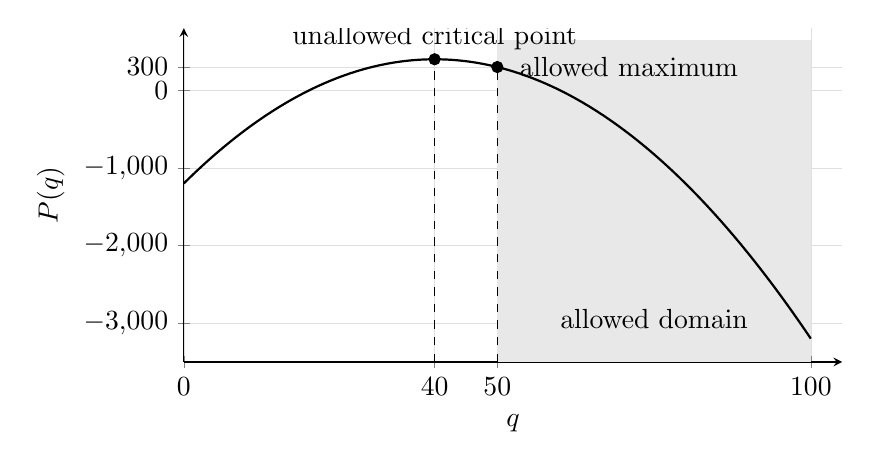
\begin{tikzpicture}
\begin{axis}[
    width=0.82\textwidth,
    height=0.48\textwidth,
    xmin=0, xmax=105,
    ymin=-3500, ymax=800,
    axis lines=left,
    xlabel={\(q\)},
    ylabel={\(P(q)\)},
    xtick={0,40,50,100},
    ytick={-3000,-2000,-1000,0,300},
    grid=both,
    grid style={line width=.1pt, draw=gray!25},
]
\path[fill=gray!18] (axis cs:50,-3500) rectangle (axis cs:100,650);
\addplot[thick, domain=0:100, samples=200] {-x^2+80*x-1200};
\addplot[only marks, mark=*] coordinates {(40,400) (50,300)};
\draw[dashed] (axis cs:40,-3500) -- (axis cs:40,400);
\draw[dashed] (axis cs:50,-3500) -- (axis cs:50,300);
\node[anchor=south] at (axis cs:40,400) {unallowed critical point};
\node[anchor=west] at (axis cs:52,300) {allowed maximum};
\node[anchor=south] at (axis cs:75,-3200) {allowed domain};
\end{axis}
\end{tikzpicture}
\caption{The critical point \(q=40\) maximizes the formula on a larger domain, but it is not an allowed production level.}
\label{fig:critical-point-outside-domain}
\end{figure}

\begin{quote}
\textbf{Moral.}

A critical point outside the physical domain is not a possible answer.  The domain is
part of the model.
\end{quote}

\subsection{A local maximum that is not the absolute maximum}
\label{subsec:local-max-not-absolute}

A local maximum is a high point nearby.  An absolute maximum is a high point
everywhere in the domain.

Those are different ideas.

Consider

\[
f(x)=x^3-3x
\]

on the interval

\[
[-2,3].
\]

Differentiate:

\[
f'(x)=3x^2-3=3(x-1)(x+1).
\]

The critical numbers are

\[
x=-1
\qquad\text{and}\qquad
x=1.
\]

The derivative is positive on \((-\infty,-1)\), negative on \((-1,1)\), and positive
on \((1,\infty)\).  Therefore \(x=-1\) is a local maximum, and \(x=1\) is a local
minimum.

Now check the values that matter for the absolute maximum on \([-2,3]\):

\[
f(-2)=-8+6=-2,
\]

\[
f(-1)=-1+3=2,
\]

\[
f(1)=1-3=-2,
\]

and

\[
f(3)=27-9=18.
\]

The local maximum value is

\[
f(-1)=2.
\]

But the absolute maximum value is

\[
f(3)=18.
\]

So the local maximum is not the absolute maximum.

\begin{figure}[h]
\centering
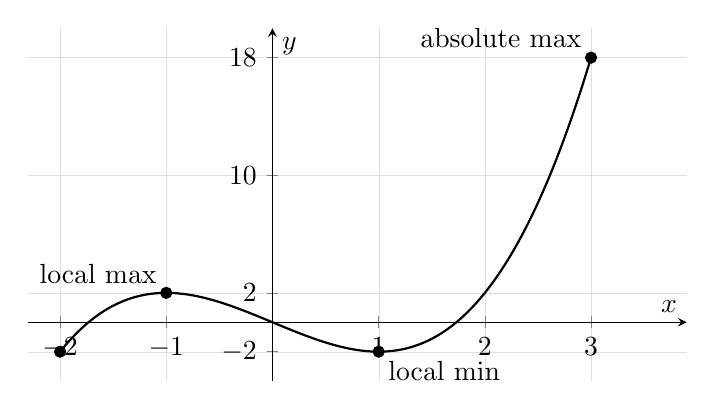
\begin{tikzpicture}
\begin{axis}[
    width=0.82\textwidth,
    height=0.50\textwidth,
    xmin=-2.3, xmax=3.9,
    ymin=-4, ymax=20,
    axis lines=middle,
    xlabel={\(x\)},
    ylabel={\(y\)},
    xtick={-2,-1,0,1,2,3},
    ytick={-2,0,2,10,18},
    grid=both,
    grid style={line width=.1pt, draw=gray!25},
]
\addplot[thick, domain=-2:3, samples=200] {x^3-3*x};
\addplot[only marks, mark=*] coordinates {(-2,-2) (-1,2) (1,-2) (3,18)};
\node[anchor=south east] at (axis cs:-1,2) {local max};
\node[anchor=north west] at (axis cs:1,-2) {local min};
\node[anchor=south east] at (axis cs:3,18) {absolute max};
\end{axis}
\end{tikzpicture}
\caption{A local high point can lose to an endpoint or to another part of the graph.}
\label{fig:local-max-not-absolute}
\end{figure}

\begin{quote}
\textbf{Moral.}

A local maximum is not automatically an absolute maximum.  For absolute extrema on
a closed interval, check all candidates: interior critical points and endpoints.
\end{quote}

\subsection{Newton's method can find the wrong root}
\label{subsec:newton-wrong-root}

Newton's method follows tangent lines.  A tangent line can cross the \(x\)-axis far
from the root we had in mind.

Consider

\[
f(x)=x^3-4x.
\]

The roots are

\[
-2,\quad 0,\quad 2.
\]

Suppose we want to find the positive root \(2\), and we start with

\[
x_0=1.
\]

Newton's method uses

\[
x_{n+1}=x_n-\frac{f(x_n)}{f'(x_n)}.
\]

Here

\[
f'(x)=3x^2-4.
\]

At \(x_0=1\),

\[
f(1)=1-4=-3,
\]

and

\[
f'(1)=3-4=-1.
\]

So

\[
x_1
=
1-\frac{-3}{-1}
=
1-3
=
-2.
\]

The method lands exactly on the root

\[
-2.
\]

That is a root of the equation, but not the root we intended to find.

\begin{figure}[h]
\centering
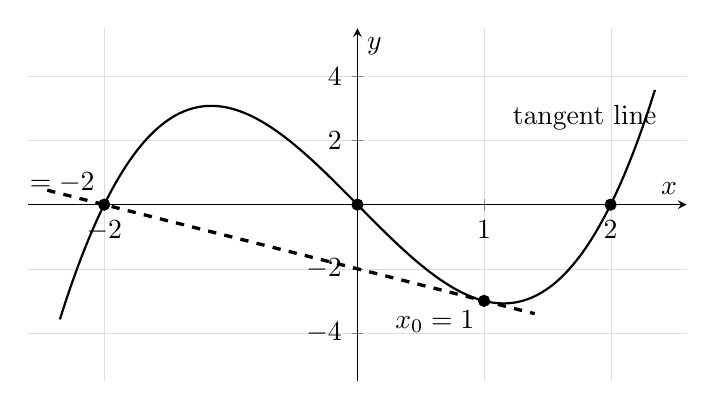
\begin{tikzpicture}
\begin{axis}[
    width=0.82\textwidth,
    height=0.50\textwidth,
    xmin=-2.6, xmax=2.6,
    ymin=-5.5, ymax=5.5,
    axis lines=middle,
    xlabel={\(x\)},
    ylabel={\(y\)},
    xtick={-2,0,1,2},
    ytick={-4,-2,0,2,4},
    grid=both,
    grid style={line width=.1pt, draw=gray!25},
]
\addplot[thick, domain=-2.35:2.35, samples=250] {x^3-4*x};
\addplot[very thick, dashed, domain=-2.45:1.4, samples=2] {-x-2};
\addplot[only marks, mark=*] coordinates {(1,-3) (-2,0) (0,0) (2,0)};
\node[anchor=north east] at (axis cs:1,-3) {\(x_0=1\)};
\node[anchor=south east] at (axis cs:-2,0) {\(x_1=-2\)};
\node[anchor=west] at (axis cs:1.15,2.7) {tangent line};
\end{axis}
\end{tikzpicture}
\caption{The tangent line at \(x_0=1\) crosses the axis at the root \(-2\), not at the intended root \(2\).}
\label{fig:newton-wrong-root}
\end{figure}

\begin{quote}
\textbf{Moral.}

Newton's method is local.  A starting point that seems reasonable may still lead to a
different root.
\end{quote}

Bracketing can help.  If the goal is the root \(2\), we can first isolate it by checking
signs on an interval such as

\[
[1,3],
\]

where

\[
f(1)<0
\qquad\text{and}\qquad
f(3)>0.
\]

Then we can monitor whether Newton's iterates remain near the intended interval.

\subsection{Newton's method may not converge}
\label{subsec:newton-no-convergence-warning}

Sometimes Newton's method does not merely find the wrong root.  Sometimes it does
not settle down at all.

Consider

\[
f(x)=x^3-2x+2.
\]

Then

\[
f'(x)=3x^2-2.
\]

Start with

\[
x_0=0.
\]

The first Newton step gives

\[
x_1
=
0-\frac{f(0)}{f'(0)}
=
0-\frac{2}{-2}
=
1.
\]

Now compute the next step:

\[
x_2
=
1-\frac{f(1)}{f'(1)}.
\]

Since

\[
f(1)=1-2+2=1
\]

and

\[
f'(1)=3-2=1,
\]

we get

\[
x_2=1-\frac11=0.
\]

So the method repeats:

\[
0,\ 1,\ 0,\ 1,\ 0,\ 1,\ldots
\]

It never converges.

The function does have a real root.  For example,

\[
f(-2)=-8+4+2=-2,
\]

while

\[
f(-1)=-1+2+2=3.
\]

By the Intermediate Value Theorem, a root lies between \(-2\) and \(-1\).  Newton's
method did not fail because no root exists.  It failed because the starting point made
the tangent process cycle.

\begin{quote}
\textbf{Moral.}

Newton's method needs a good starting point and a nonzero derivative.  It is fast when
it behaves well, but it is not guaranteed to behave well from every starting point.
\end{quote}

\subsection{The common lesson}
\label{subsec:common-lesson-warning-examples}

The warning examples have one message:

\[
\boxed{
\text{A calculus method is only as good as the question it is applied to.}
}
\]

Before trusting an answer, ask:

\[
\begin{array}{ll}
\text{1.} & \text{Is the candidate inside the physical domain?}\\
\text{2.} & \text{Have the endpoints been checked?}\\
\text{3.} & \text{Is the result local or absolute?}\\
\text{4.} & \text{Does the sign or unit of the answer make sense?}\\
\text{5.} & \text{For Newton's method, do the iterates stabilize and is \(f(x_n)\) small?}
\end{array}
\]

\section{Chapter review and applications}
\label{sec:chapter7-review-applications}

This chapter began with a simple change in perspective.  Instead of being handed a
function and asked to differentiate it, we were asked to build the function first.

A ladder slides.  A box is folded.  A cup cools.  A population grows.  A light ray
chooses a path.  In each case, the derivative did not appear at the beginning.  It
appeared after we translated the situation into mathematics.

That is the main skill of the chapter:

\[
\text{real situation}
\quad\longrightarrow\quad
\text{mathematical model}
\quad\longrightarrow\quad
\text{derivative information}
\quad\longrightarrow\quad
\text{interpretation}.
\]

The last step is as important as the first.  A derivative answer without units, sign,
domain, and meaning is not yet an answer to the problem.

\subsection{The chapter in one map}
\label{subsec:chapter7-one-map}

The chapter used derivatives in several different ways.  The same derivative idea
kept returning with different names.

\[
\begin{array}{c|c|c}
\textbf{topic} & \textbf{main question} & \textbf{derivative role} \\ \hline
\text{related rates} & \text{How fast is one quantity changing?}
& \text{differentiate a relation} \\[4pt]
\text{optimization} & \text{Which choice is best?}
& \text{find and test candidates} \\[4pt]
\text{linear approximation} & \text{How much does the output change?}
& \Delta y\approx f'(x)\Delta x \\[4pt]
\text{Newton's method} & \text{Where is a zero?}
& \text{use tangent-line correction} \\[4pt]
\text{exponential models} & \text{What grows at a rate proportional to itself?}
& y'=ky \\[4pt]
\text{logistic models} & \text{How does growth slow near a limit?}
& P'=rP\left(1-\dfrac{P}{K}\right) \\[8pt]
\text{least-time paths} & \text{Which path makes time stationary?}
& \text{differentiate time or distance}
\end{array}
\]

\begin{figure}[h]
\centering
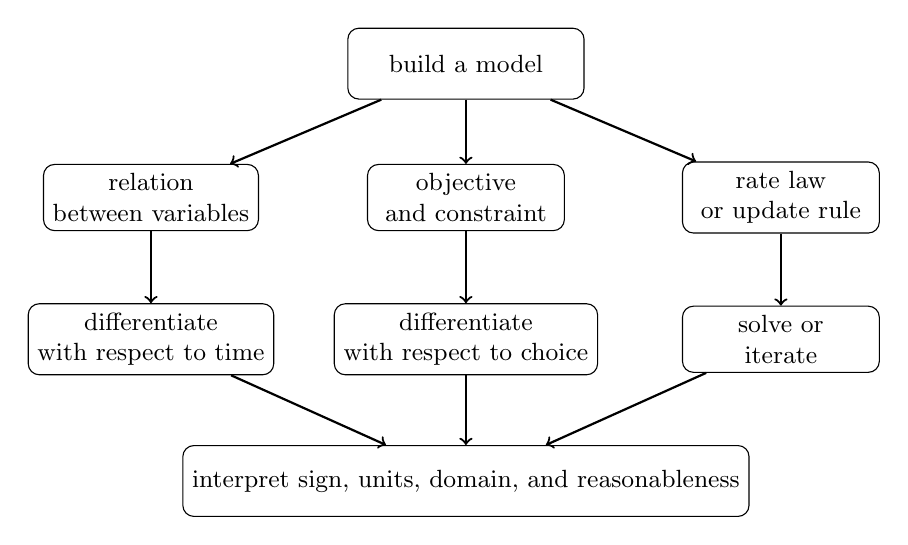
\begin{tikzpicture}[
  box/.style={draw, rounded corners, align=center, minimum width=3.0cm, minimum height=0.9cm},
  smallbox/.style={draw, rounded corners, align=center, minimum width=2.5cm, minimum height=0.78cm},
  every node/.style={font=\small}
]
  \node[box] (model) at (0,0) {build a model};
  \node[smallbox] (relation) at (-4,-1.7) {relation\\between variables};
  \node[smallbox] (objective) at (0,-1.7) {objective\\and constraint};
  \node[smallbox] (law) at (4,-1.7) {rate law\\or update rule};

  \node[smallbox] (differentiate) at (-4,-3.5) {differentiate\\with respect to time};
  \node[smallbox] (optimize) at (0,-3.5) {differentiate\\with respect to choice};
  \node[smallbox] (solve) at (4,-3.5) {solve or\\iterate};

  \node[box] (interpret) at (0,-5.3) {interpret sign, units, domain, and reasonableness};

  \draw[->, thick] (model) -- (relation);
  \draw[->, thick] (model) -- (objective);
  \draw[->, thick] (model) -- (law);

  \draw[->, thick] (relation) -- (differentiate);
  \draw[->, thick] (objective) -- (optimize);
  \draw[->, thick] (law) -- (solve);

  \draw[->, thick] (differentiate) -- (interpret);
  \draw[->, thick] (optimize) -- (interpret);
  \draw[->, thick] (solve) -- (interpret);
\end{tikzpicture}
\caption{The chapter's methods all follow the same modeling path: translate, differentiate, solve, and interpret.}
\label{fig:chapter7-model-map}
\end{figure}

\begin{quote}
\textbf{A derivative answer must still pass three checks.}

\[
\text{Does the sign make sense?}
\]

\[
\text{Do the units make sense?}
\]

\[
\text{Is the answer allowed by the domain of the model?}
\]
\end{quote}

These checks are not afterthoughts.  They are part of the mathematics.

\subsection{Formulas to remember}
\label{subsec:chapter7-formulas}

The formulas below are not separate tricks.  Each is a compact version of an idea from
the chapter.

\[
\begin{array}{c|c}
\textbf{idea} & \textbf{formula} \\ \hline
\text{linear approximation} &
f(a+\Delta x)\approx f(a)+f'(a)\Delta x \\[6pt]
\text{differential estimate} &
dy=f'(x)\,dx \\[6pt]
\text{Newton's method} &
x_{n+1}=x_n-\dfrac{f(x_n)}{f'(x_n)} \\[12pt]
\text{exponential growth or decay} &
y'=ky,\qquad y(t)=y_0e^{kt} \\[8pt]
\text{doubling time} &
D=\dfrac{\ln2}{k}\quad(k>0) \\[10pt]
\text{half-life} &
H=-\dfrac{\ln2}{k}\quad(k<0) \\[10pt]
\text{Newton's law of cooling} &
T(t)=T_s+\bigl(T(0)-T_s\bigr)e^{-kt} \\[8pt]
\text{logistic growth} &
P'=rP\left(1-\dfrac{P}{K}\right) \\[12pt]
\text{logistic solution} &
P(t)=\dfrac{K}{1+\left(\dfrac{K-P_0}{P_0}\right)e^{-rt}}
\end{array}
\]

For related rates and optimization, the most important formulas are often not fixed in
advance.  The formula comes from the geometry or the constraint.

A ladder problem uses

\[
x^2+y^2=L^2.
\]

A cone problem uses

\[
V=\frac13\pi r^2h
\]

together with similar triangles.  A box problem uses a volume formula and a physical
domain.  A can problem uses surface area and a fixed-volume constraint.

The hard part is not memorizing formulas.  The hard part is choosing the right
quantities and keeping the model honest.

\subsection{Skills: related rates and optimization}
\label{subsec:skills-related-rates-optimization}

Related rates and optimization are the two main problem-solving skills of this chapter.
They look similar because both begin with translation, but they ask different questions.

\[
\begin{array}{c|c|c}
\textbf{problem type} & \textbf{what changes?} & \textbf{what is the goal?} \\ \hline
\text{related rates} & \text{quantities change with time} & \text{find an unknown rate} \\[4pt]
\text{optimization} & \text{a choice variable changes} & \text{maximize or minimize a quantity}
\end{array}
\]

\paragraph{Related rates checklist.}

\[
\begin{array}{ll}
\text{1.} & \text{Draw a picture, if geometry is involved.}\\
\text{2.} & \text{Name the changing quantities as functions of time.}\\
\text{3.} & \text{Write an equation relating the quantities.}\\
\text{4.} & \text{Differentiate with respect to time.}\\
\text{5.} & \text{Substitute values for the instant in question.}\\
\text{6.} & \text{Solve for the desired rate.}\\
\text{7.} & \text{Check sign and units.}
\end{array}
\]

The most common mistake is substituting the instant-specific numbers too early.  The
variables must remain variables until after the relation has been differentiated.

\paragraph{Optimization checklist.}

\[
\begin{array}{ll}
\text{1.} & \text{Name the quantity to optimize.}\\
\text{2.} & \text{Name the variables.}\\
\text{3.} & \text{Write the objective function.}\\
\text{4.} & \text{Write the constraint.}\\
\text{5.} & \text{Use the constraint to get one variable.}\\
\text{6.} & \text{Find the physical domain.}\\
\text{7.} & \text{Find critical numbers and check endpoints.}\\
\text{8.} & \text{Translate the result back into the situation.}
\end{array}
\]

The most common mistake is finding a critical point and stopping.  A critical point is
a candidate, not a conclusion.

\subsection{Review problems}
\label{subsec:chapter7-review-problems}

The problems below are meant to mix the chapter's ideas.  For each one, write a complete
solution with units and a sentence interpreting the answer.

\begin{enumerate}
\item \textbf{Inflating sphere.}
Air is pumped into a spherical balloon at a constant rate of

\[
30\pi\text{ cm}^3/\text{s}.
\]

How fast is the radius increasing when the radius is \(5\) cm?

\item \textbf{Sliding ladder.}
A \(13\)-foot ladder leans against a wall.  The bottom slides away from the wall at

\[
3\text{ ft/s}.
\]

How fast is the top sliding down when the bottom is \(5\) feet from the wall?

\item \textbf{Water in a cone.}
An inverted cone has height \(10\) feet and radius \(5\) feet at the top.  Water is
flowing in at

\[
3\text{ ft}^3/\text{min}.
\]

How fast is the water level rising when the water height is \(4\) feet?

\item \textbf{Two cars.}
One car travels east from an intersection at \(40\) mph.  Another travels north from
the same intersection at \(30\) mph.  How fast is the distance between the cars
increasing \(2\) hours later?

\item \textbf{Largest rectangle under a parabola.}
A rectangle has its base on the \(x\)-axis and its upper two vertices on the graph

\[
y=12-x^2.
\]

Assume the rectangle is symmetric about the \(y\)-axis.  What dimensions give the
largest area?

\item \textbf{Open box.}
A \(20\)-inch by \(30\)-inch sheet of cardboard has equal squares of side length \(x\)
cut from its corners.  The sides are folded up to make an open box.  What value of
\(x\) gives the largest volume?

\item \textbf{Fence along a river.}
A farmer has \(300\) meters of fencing and wants to make a rectangular field along
a river, using the river as one side.  What dimensions maximize the area?

\item \textbf{Least material can.}
A closed cylindrical can must hold

\[
1000\text{ cm}^3.
\]

Ignoring seams and thickness, find the radius and height that minimize surface area.

\item \textbf{Newton's method.}
Use Newton's method to approximate the positive solution of

\[
x^3=10.
\]

Start with \(x_0=2\).  Compute \(x_1\), \(x_2\), and \(x_3\).

\item \textbf{Cooling model.}
A metal object is heated to \(100^\circ\text{C}\) and placed in a room at
\(20^\circ\text{C}\).  After \(5\) minutes, its temperature is \(70^\circ\text{C}\).
Assuming Newton's law of cooling, estimate its temperature after \(15\) minutes.

\item \textbf{Logistic growth.}
A population satisfies

\[
P'=0.6P\left(1-\frac{P}{800}\right),
\qquad
P(0)=100.
\]

Find \(P(t)\).  When does the population reach \(400\)?

\item \textbf{A warning problem.}
A model for profit is

\[
P(q)=-q^2+60q-500.
\]

A factory is allowed to produce only

\[
40\le q\le 80
\]

units.  Find the production level that maximizes profit on the allowed domain.
Explain why the unconstrained critical point is not the answer.
\end{enumerate}

\subsection{Project: design a least-material container}
\label{subsec:project-least-material-container}

A basic can problem assumes that all material costs the same.  Real containers are
not always like that.  The top and bottom may need thicker material.  The side wall
may be cheaper.  The seams may matter.

This project keeps the model simple but makes the design question more realistic.

\paragraph{Design brief.}
A closed cylindrical container must hold a fixed volume

\[
V_0
\]

cubic centimeters.  The side wall costs \(1\) unit per square centimeter.  The top and
bottom cost \(c\) units per square centimeter, where

\[
c>0.
\]

Find the radius and height that minimize material cost.

\begin{figure}[h]
\centering
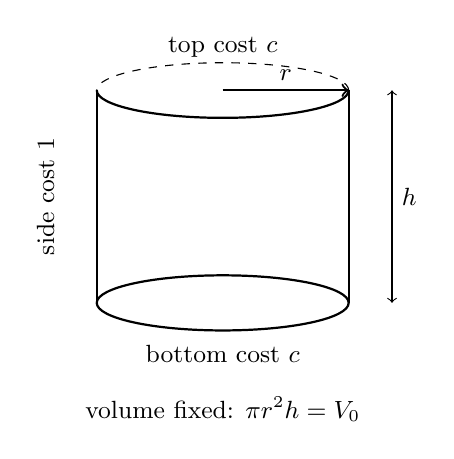
\begin{tikzpicture}[scale=1.0, every node/.style={font=\small}]
  % cylinder
  \draw[thick] (-1.6,1.3) arc[start angle=180,end angle=360,x radius=1.6,y radius=0.35];
  \draw[dashed] (1.6,1.3) arc[start angle=0,end angle=180,x radius=1.6,y radius=0.35];
  \draw[thick] (-1.6,-1.4) arc[start angle=180,end angle=360,x radius=1.6,y radius=0.35];
  \draw[thick] (-1.6,-1.4) arc[start angle=180,end angle=0,x radius=1.6,y radius=0.35];
  \draw[thick] (-1.6,1.3) -- (-1.6,-1.4);
  \draw[thick] (1.6,1.3) -- (1.6,-1.4);

  % radius and height labels
  \draw[->, thick] (0,1.3) -- (1.6,1.3);
  \node[above] at (0.8,1.3) {\(r\)};

  \draw[<->] (2.15,1.3) -- (2.15,-1.4);
  \node[right] at (2.15,-0.05) {\(h\)};

  % cost labels
  \node at (0,1.85) {top cost \(c\)};
  \node at (0,-2.05) {bottom cost \(c\)};
  \node[rotate=90] at (-2.25,-0.05) {side cost \(1\)};

  \node at (0,-2.75) {volume fixed: \(\pi r^2h=V_0\)};
\end{tikzpicture}
\caption{A more realistic container model can assign different costs to the side wall and the two circular ends.}
\label{fig:least-material-container-project}
\end{figure}

\paragraph{Step 1: Build the cost function.}
The side area is

\[
2\pi rh.
\]

The top and bottom together have area

\[
2\pi r^2.
\]

Since the top and bottom cost \(c\) units per square centimeter, the material cost is

\[
M=2\pi rh+2c\pi r^2.
\]

The volume constraint is

\[
\pi r^2h=V_0.
\]

Solve the constraint for \(h\):

\[
h=\frac{V_0}{\pi r^2}.
\]

Substitute into the cost:

\[
M(r)
=
2\pi r\left(\frac{V_0}{\pi r^2}\right)+2c\pi r^2.
\]

Thus

\[
M(r)=\frac{2V_0}{r}+2c\pi r^2,
\qquad r>0.
\]

\paragraph{Step 2: Minimize.}
Differentiate:

\[
M'(r)=-\frac{2V_0}{r^2}+4c\pi r.
\]

Set \(M'(r)=0\):

\[
-\frac{2V_0}{r^2}+4c\pi r=0.
\]

Multiply by \(r^2\):

\[
-2V_0+4c\pi r^3=0.
\]

So

\[
4c\pi r^3=2V_0,
\]

and therefore

\[
r^3=\frac{V_0}{2c\pi}.
\]

Thus

\[
\boxed{
r=\left(\frac{V_0}{2c\pi}\right)^{1/3}.
}
\]

Now find the height:

\[
h=\frac{V_0}{\pi r^2}.
\]

Since

\[
V_0=2c\pi r^3,
\]

we get

\[
h=\frac{2c\pi r^3}{\pi r^2}=2cr.
\]

Therefore the optimal shape satisfies

\[
\boxed{
h=2cr.
}
\]

When \(c=1\), this gives

\[
h=2r.
\]

So the height equals the diameter, which matches the equal-cost can from Section
\ref{subsec:geometry-optimization}.

\paragraph{Step 3: Interpret the parameter \(c\).}
The ratio

\[
\frac{h}{r}=2c
\]

shows how the design changes with material cost.

\[
\begin{array}{c|c|c}
c & h/r & \text{interpretation} \\ \hline
1 & 2 & \text{height equals diameter} \\
2 & 4 & \text{top and bottom are expensive, so use smaller ends} \\
4 & 8 & \text{ends are very expensive, so make the can tall and narrow}
\end{array}
\]

The formula tells a physical story.  If the circular ends are expensive, the design tries
to reduce their area by using a smaller radius.  To keep the same volume, the height
must increase.

\paragraph{Report questions.}
Write a short report answering these questions.

\begin{enumerate}
\item Derive the cost function \(M(r)\) from the geometry and the volume constraint.

\item Prove that the critical point gives an absolute minimum.  One way is to use

\[
M''(r)=\frac{4V_0}{r^3}+4c\pi>0.
\]

Another way is to examine what happens to \(M(r)\) as \(r\to0^+\) and as
\(r\to\infty\).

\item For

\[
V_0=1000\text{ cm}^3
\]

compute the optimal \(r\) and \(h\) for

\[
c=1,\qquad c=2,\qquad c=4.
\]

\item Make a graph of \(M(r)\) for each value of \(c\).  Mark the minimizing radius.

\item Explain, in words, why increasing \(c\) makes the optimal container taller and
narrower.

\item Extension.  Suppose the container has no top.  If the bottom costs \(c\) units per
square centimeter and the side costs \(1\), build and minimize the new cost function.
\end{enumerate}

\subsection{Project: model cooling data}
\label{subsec:project-model-cooling-data}

Chapter 2 used cooling coffee as an example of data that should not be modeled by a
line forever.  This chapter gives the derivative law behind the better model.

Newton's law of cooling says

\[
T'=-k(T-T_s),
\qquad k>0,
\]

where \(T_s\) is the surrounding temperature.  The solution is

\[
T(t)=T_s+\bigl(T(0)-T_s\bigr)e^{-kt}.
\]

The quantity that decays exponentially is not \(T\) itself.  It is the excess temperature

\[
T-T_s.
\]

\paragraph{Data.}
A cup of coffee sits in a room whose temperature is

\[
22^\circ\text{C}.
\]

The measured temperatures are:

\[
\begin{array}{c|cccccc}
t\text{ (minutes)} & 0 & 5 & 10 & 15 & 20 & 25 \\ \hline
T(t)\text{ }(^\circ\text{C}) & 90 & 73 & 60 & 51 & 44 & 39
\end{array}
\]

\begin{figure}[h]
\centering
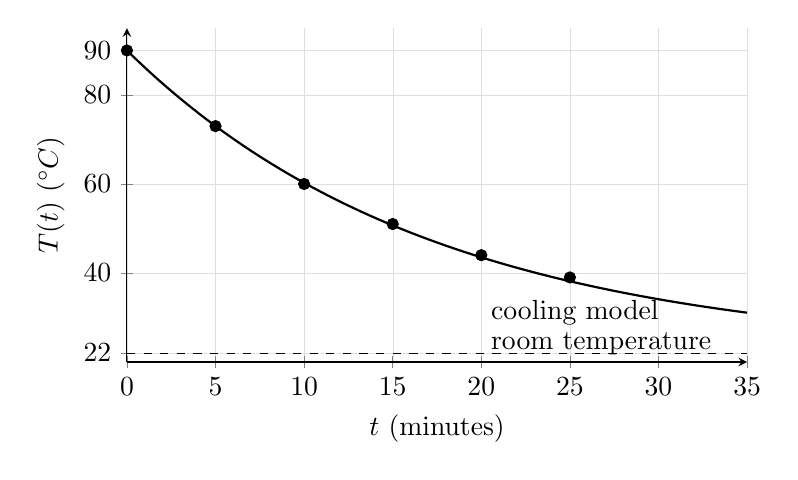
\begin{tikzpicture}
\begin{axis}[
    width=0.78\textwidth,
    height=0.48\textwidth,
    xmin=0, xmax=35,
    ymin=20, ymax=95,
    axis lines=left,
    xlabel={\(t\) (minutes)},
    ylabel={\(T(t)\) (\(^\circ\text{C}\))},
    xtick={0,5,10,15,20,25,30,35},
    ytick={22,40,60,80,90},
    grid=both,
    grid style={line width=.1pt, draw=gray!25},
]
\addplot[only marks, mark=*] coordinates {
    (0,90) (5,73) (10,60) (15,51) (20,44) (25,39)
};
\addplot[thick, domain=0:35, samples=200] {22+68*exp(-0.057536*x)};
\addplot[dashed, domain=0:35, samples=2] {22};
\node[anchor=west] at (axis cs:20,31) {cooling model};
\node[anchor=west] at (axis cs:20,24) {room temperature};
\end{axis}
\end{tikzpicture}
\caption{Newton's law of cooling models the excess temperature \(T-22\) as exponential decay.}
\label{fig:cooling-data-project}
\end{figure}

\paragraph{A first model from two points.}
Since

\[
T_s=22
\]

and

\[
T(0)=90,
\]

the model has the form

\[
T(t)=22+68e^{-kt}.
\]

Use \(T(5)=73\):

\[
73=22+68e^{-5k}.
\]

Thus

\[
51=68e^{-5k},
\]

so

\[
e^{-5k}=\frac{51}{68}=\frac34.
\]

Therefore

\[
k=-\frac15\ln\left(\frac34\right).
\]

Numerically,

\[
k\approx0.0575.
\]

So a two-point model is

\[
\boxed{
T(t)=22+68e^{-0.0575t}.
}
\]

Equivalently,

\[
T(t)=22+68\left(\frac34\right)^{t/5}.
\]

This form says that every \(5\) minutes, the excess temperature is multiplied by
about \(3/4\).

\paragraph{Prediction.}
The predicted temperature after \(30\) minutes is

\[
T(30)=22+68\left(\frac34\right)^6.
\]

Since

\[
\left(\frac34\right)^6\approx0.178,
\]

we get

\[
T(30)\approx22+68(0.178)\approx34.1^\circ\text{C}.
\]

\paragraph{Computing task.}
The two-point model uses only the first two measurements.  A better model should
use all the data.

Let

\[
E(t)=T(t)-22
\]

be the excess temperature.  If Newton's law is a good model, then

\[
E(t)=E(0)e^{-kt}.
\]

Taking natural logarithms gives

\[
\ln E(t)=\ln E(0)-kt.
\]

So the points

\[
\bigl(t,\ln(T(t)-22)\bigr)
\]

should lie approximately on a line with slope \(-k\).

Complete the following tasks.

\begin{enumerate}
\item Compute the excess temperatures \(E(t)=T(t)-22\).

\item Compute \(\ln E(t)\) for each measured time.

\item Plot the points

\[
(t,\ln E(t)).
\]

Do they look approximately linear?

\item Estimate the slope of the best-fitting line.  Then estimate

\[
k=-\text{slope}.
\]

\item Build the model

\[
T(t)=22+Ae^{-kt}.
\]

You may take \(A=68\), or estimate \(A\) from your fitted line.

\item Use your model to predict \(T(30)\), \(T(45)\), and \(T(60)\).

\item Compute residuals:

\[
\text{residual}
=
\text{measured temperature}
-
\text{model temperature}.
\]

Are the residuals small?  Do they show a pattern?

\item Compare the cooling model with the linear model through the first and last
data points.  Which model gives a more reasonable prediction after \(2\) hours?
Explain.
\end{enumerate}

\begin{quote}
\textbf{What the project tests.}

A model is not only a formula that fits numbers.  It should also respect the behavior
of the situation.  A cooling object should approach room temperature, not pass below
it because a line keeps decreasing forever.
\end{quote}

\subsection{Concept checks}
\label{subsec:chapter7-concept-checks}

\begin{enumerate}
\item In a related rates problem, why should we usually differentiate before substituting
the values for the instant in question?

\item In an optimization problem, why is the physical domain part of the model?

\item A critical point of an objective function lies outside the physical domain.  What
should you do with it?

\item Explain the difference between absolute error and relative error.

\item Why does Newton's method require \(f'(x_n)\neq0\)?

\item Give one reason Newton's method can fail even when a root exists.

\item In the equation

\[
y'=ky,
\]

what does \(k\) measure?

\item Why is

\[
P'=rP\left(1-\frac{P}{K}\right)
\]

approximately exponential when \(P\ll K\)?

\item In the logistic model, why is the growth fastest at \(P=K/2\)?

\item Reflection minimizes distance, but refraction minimizes time.  Why are these not
the same problem when the speed changes?
\end{enumerate}

\subsection{Where this points}
\label{subsec:chapter7-hook-integrals}

This chapter showed how much can be done with a derivative.

A derivative can relate changing quantities.  It can find a best choice.  It can estimate
error.  It can turn a tangent line into a root-finding method.  It can express a physical
law such as

\[
T'=-k(T-T_s)
\]

or

\[
P'=rP\left(1-\frac{P}{K}\right).
\]

But a derivative is still local.  It tells how fast something is changing at an instant.

Many questions ask for the accumulated result of those changes.

If velocity is known at every instant, how far did the object travel?

If a force changes with position, how much work was done?

If density varies along a rod, what is the rod's total mass?

If a rate law tells how a quantity changes, how much total change has occurred over
an interval?

Those questions return us to the dashboard from the beginning of the book.  The
speedometer gives rate.  The odometer gives accumulation.

The next chapter builds the second great operation of calculus: adding up infinitely
many small changes.
